\documentclass[a4paper]{scrartcl}

\usepackage[
fancytheorems, 
fancyproofs, 
noindent, 
%  spacingfix,  
]{adam}


\usepackage{bm}
\usepackage{tikz}
\newcommand{\hh}[1]{\hat{\vv{#1}}}

\allowdisplaybreaks

\title{Dynamics and Relativity}
\author{Adam Kelly (\texttt{ak2316@cam.ac.uk})}
\date{\today} 
 
\begin{document}

\maketitle  

Dynamics and relativity sets the scene for studying the problems of Newtonian dynamics and, towards the end, Einstein's theory of special relativity.

The first part of this course develops \emph{Newtonian mechanics} -- a mathematical framework built around the notion of a force, which turns out to be capable of describing an astonishing range of physical phenomena: projectiles, oscillations, planetary orbits, spinning tops and much more. Along the way we will meet the great conserved quantities of physics (energy, momentum and angular momentum), and we will see how symmetry principles constrain what a physical law is allowed to look like. The second part of the course takes one such symmetry principle seriously enough to break Newtonian mechanics entirely: insisting that the speed of light is the same for all observers leads to \emph{special relativity}, where space and time mix together, moving clocks run slow, and mass is just another form of energy.

This article constitutes my notes for the `Dynamics and Relativity' course, held in Lent 2021 at Cambridge. These notes are \emph{not a transcription of the lectures}, and differ significantly in quite a few areas. Still, all lectured material should be covered.

\tableofcontents

\section{Newton's Laws and Forces}


In Newtonian mechanics, we use the idea of a force to build up a mathematical framework in which we can describe the motion of objects, typically particles.

\subsection{Particles \& Inertial Frames}

Newtonian mechanics is at its cleanest when describing the motion of \emph{particles}.

\begin{definition}[Particle]
	A \vocab{particle} is an idealised object of negligible size and no internal structure, to which we can assign physical properties such as mass $m > 0$ and electric charge $q$.
\end{definition}

Real objects are, of course, not points. This idealisation is still tremendously useful for two reasons. First, an extended body can be treated as a particle whenever its size is irrelevant to the problem at hand -- the Earth, viewed on the scale of the solar system, is quite point-like. Secondly, as we will see in Section~\ref{sec:systems}, an extended body can be modelled as a large collection of particles, and its overall motion is then governed by the very same laws.

To describe the positions of particles over time, we use a \emph{reference frame}, which consists of a choice of origin and some coordinate system which can be used to consistently describe position.

For a particle with position vector $\vv x(t)$, a displacement vector from the origin of our reference frame, we then define the following quantities.
\begin{itemize}
	\item \emph{Velocity}. The velocity $\vv v$ of the particle is $\vv v = \dot{\vv x} = \dd \vv x(t) / \dd t$. This vector is always tangent to the particle's trajectory. The speed is then $v = |\vv v|$.
	\item \emph{Acceleration}. The acceleration $\vv a$ of a particle is $\vv a = \ddot{\vv x} = \dd^2 \vv x(t)/\dd t^2$.
	\item \emph{Momentum}. The momentum $\vv p$ is then $\vv p = m \vv v = m \dot{\vv x}$.
\end{itemize}
Throughout these notes, an overdot will always denote a derivative with respect to time.

\subsection{Newton's Laws}

The whole of Newtonian mechanics rests on three laws, which we will treat as axioms of our theory.

\begin{law}[Newton's Laws of Motion]
	\begin{enumerate}
		\item \emph{Galileo's Law of Inertia}. There exist \vocab{inertial frames}, reference frames in which particles travel at constant velocity when the force acting on them vanishes.
		\item \emph{Newton's Second Law}. If a force $\vv F$ acts on a particle with momentum $\vv p$, then $\dd\vv p/\dd t = \vv F$.
		\item \emph{Newton's Third Law}. Every action has an equal and opposite reaction: if a particle $A$ exerts a force $\vv F$ on a particle $B$, then $B$ exerts a force $-\vv F$ on $A$.
	\end{enumerate}
\end{law}

All of these are tied together with the \emph{principle of Galilean relativity}, which is that the laws of physics are the same in every inertial reference frame.

A few comments are in order. The first law looks at a glance like it is just a special case of the second (if $\vv F = \vv 0$ then $\vv p$ is constant) -- its actual content is the \emph{existence} of inertial frames, which is what makes the second law meaningful at all. A frame fixed to a spinning roundabout is not inertial: a particle with no force on it will appear to accelerate. Throughout the Newtonian part of this course we will work in inertial frames unless stated otherwise (and we will study what happens in rotating, non-inertial frames in Section~\ref{sec:rotating}).

For a particle whose mass is constant, the second law reads
$$
m \ddot{\vv x} = \vv F(\vv x, \dot{\vv x}, t),
$$
which is a second order ordinary differential equation for the trajectory $\vv x(t)$. Assuming the force is well behaved, such an equation has a unique solution once we specify the initial position $\vv x(t_0)$ and initial velocity $\dot{\vv x}(t_0)$. This is worth dwelling on -- it means Newtonian mechanics is \emph{deterministic}: the position and velocity of a particle right now determine its entire future (and past) motion. Solving dynamics problems is therefore really the art of solving differential equations.

\subsection{Galilean Transformations}

A natural question is how one can transform between different inertial frames. That is, under what transformations do the laws of physics remain unchanged. It is straightforward to see that if we have some $(\vv x, t)$ in an inertial frame $\FF$, then we can construct another inertial frame $\FF'$ by combining:
\begin{itemize}
	\item \emph{Translations}. $\vv x' = \vv x + \vv a$ for a constant vector $\vv a$, and $t' = t + t_0$ for a constant $t_0$.
	\item \emph{Rotations and Reflections}. $\vv x' = R \vv x$, where $R$ is some orthogonal matrix.
	\item \emph{Boosts}. $\vv x' = \vv x + \vv v t$, for a constant velocity vector $\vv v$.
\end{itemize}
This set of transformations forms the \emph{Galilean group}, the group of symmetries of Newton's laws. Indeed, each of these transformations maps straight-line motion to straight-line motion, so each maps inertial frames to inertial frames, and the general element of the group is a composition of the above types.

The principle of Galilean relativity can then be restated as: \emph{the laws of physics are invariant under Galilean transformations}. Note that any Galilean transformation has $\ddot{\vv x}' = R\ddot{\vv x}$, so a particle's acceleration is the same in all inertial frames (up to the fixed rotation of the axes). Since Newton's second law involves only acceleration, and not absolute position or absolute velocity, it is compatible with this principle -- there is no mechanical experiment that can detect a state of `absolute rest'. A passenger in a smoothly moving train can pour their tea exactly as if they were at rest.

When working with Newton's laws, we assume that there is some `absolute time', with the times $t$, $t'$ in two inertial frames differing by at most a constant\footnote{Once we fix the units, of course.}. All inertial observers therefore agree on the time interval between two events. This seems so obvious as to not be worth stating, but it is really a physical assumption -- and we will see in Section~\ref{sec:sr} that it is \emph{false} when speeds involved approach the speed of light.

\begin{example}[Projectiles on a Train]
	Let's check covariance concretely. In the frame $\FF$ of the ground, a projectile obeys $m\ddot{\vv x} = m \vv g$, giving parabolic trajectories. Now watch from the frame $\FF'$ of a train moving at constant velocity $\vv v$, so $\vv x' = \vv x - \vv v t$. Then
	$$
	\ddot{\vv x}' = \ddot{\vv x} = \vv g,
	$$
	so the equation of motion takes \emph{exactly the same form} in the train frame, and the trajectory is again a parabola -- just one with different initial conditions (the initial velocity is shifted by $-\vv v$). A ball tossed straight up on a smoothly moving train lands back in your hand, not behind you; no experiment with projectiles can reveal the train's motion. Contrast an \emph{accelerating} train: then $\ddot{\vv x}' = \vv g - \vv a$, the form of the law changes, and the tossed ball drifts backwards -- accelerated frames are detectably not inertial.
\end{example}

\subsection{Examples of Forces}

Newton's laws tell us how a particle responds to a force, but they are silent on what forces actually arise in nature -- that information must be supplied separately, by \emph{force laws}. At the fundamental level, remarkably few are needed: gravity and electromagnetism account for essentially everything we will meet in this course (the strong and weak nuclear forces operate only at subatomic ranges). The everyday `contact' forces -- tension in strings, normal reactions from surfaces, friction -- are all electromagnetic in origin, arising from the interactions of vast numbers of atoms, and we model them phenomenologically rather than from first principles.

The \emph{Lorentz force} describes the force on a particle moving in an electromagnetic field. If a particle has position $\vv x$ and charge $q$, and it moves in an electric field $\vv E$ and magnetic field $\vv B$, then the force on the particle is given by
$$
\vv F = q(\vv E + \dot{\vv x} \times \vv B).
$$


The \emph{gravitational force} describes the force due to gravity on a particle. If two particles have masses $m_1$ and $m_2$ and positions $\vv x_1$ and $\vv x_2$, then the force of gravity between them is given by
$$
\vv F_1 = - \frac{G m_1 m_2}{| \vv x_1 - \vv x_2|^3} (\vv x_1 - \vv x_2) = - \vv F_2,
$$
where $G$ is the \vocab{gravitational constant}.


\subsection{Potentials in One Dimension}

Roughly, the framework of Newtonian mechanics takes in particles and forces, and from that we get the dynamics at play. However, in many cases we think of forces as coming from a more primitive idea, one of \emph{potentials}. We will work in one dimension for the time being.

\begin{definition}[Potential Energy]
	For a force field $F(x)$, depending only on position, we define the \vocab{potential energy} to be a function $V(x)$ such that
	$$
	F = - \frac{\dd V}{\dd x},
	$$
	so $V = -\int F \dd x$, defined up to a constant.
\end{definition}

With this, Newton's second law becomes $\dot{p} = -\dd V/\dd x$. The arbitrary constant is harmless: only differences in potential energy will ever matter physically, so we may fix the constant however is convenient.

With forces in one dimension depending on position only, we have a naturally conserved quantity. We define the \emph{kinetic energy} of a particle to be $T = \frac{1}{2}m \dot{x}^2$.

\begin{proposition}[Conservation of Energy]
	Consider a particle of mass $m$ moving under a force $F(x) = -\dd V/\dd x$. Then the \vocab{total energy}
	$$
	E = T + V = \frac{1}{2}m\dot{x}^2 + V(x)
	$$
	is conserved, that is, $\dot{E} = 0$.
\end{proposition}
\begin{proof}
	Differentiating with respect to time, using the chain rule and then Newton's second law,
	$$
	\frac{\dd E}{\dd t} = m \dot{x} \ddot{x} + \frac{\dd V}{\dd x}\dot{x} = \dot{x}\left(m \ddot{x} - F(x)\right) = 0,
	$$
	as required.
\end{proof}

It is important in this proposition that $F$ depends only on position -- if $F$ depends on, say, velocity (as friction does), the argument breaks down and energy is typically not conserved.

\begin{remark}
	A theme worth watching throughout this course: conserved quantities are systematically tied to \emph{symmetries}. Energy conservation will hold when the physics is unchanged by translation in time; momentum conservation when it is unchanged by translation in space; angular momentum conservation when it is unchanged by rotation. This correspondence is made precise by \emph{Noether's theorem}, which appears properly in next year's `Variational Principles' course -- but you can already spot the pattern in every conservation law we derive.
\end{remark}

One nice thing about having such a conserved quantity is that
$$
E = \frac{1}{2}m \dot{x}^2 + V(x) \implies  \dot{x} = \pm \sqrt{\frac{2}{m} (E - V(x))},
$$
which gives us a \emph{first order} differential equation for position, which we can (at least in principle) solve by separating variables. The conservation of energy has done one integration of Newton's second law for us. Let's see this in action.

\begin{example}[The Harmonic Oscillator]
	The \vocab{harmonic oscillator} is the system with quadratic potential
	$$
	V(x) = \frac{1}{2}k x^2,
	$$
	which describes, for example, a particle attached to a spring of stiffness $k$: the force $F = -\dd V/\dd x = -kx$ is a restoring force proportional to the displacement (this is `Hooke's law').
	The equation of motion
	$$
	m \ddot{x} = -kx
	$$
	is linear, and has general solution
	$$
	x(t) = A \cos \omega t + B \sin \omega t, \quad \text{where } \omega = \sqrt{k/m}.
	$$
	The motion is periodic with \emph{angular frequency} $\omega$, that is, with period $\tau = 2\pi/\omega$. Note that the period is independent of the amplitude of the oscillation.
	Substituting the solution back in, the energy is
	$$
	E = \frac{1}{2}m\dot{x}^2 + \frac{1}{2}kx^2 = \frac{1}{2}k(A^2 + B^2),
	$$
	which is indeed constant. Energy sloshes back and forth between kinetic and potential, twice per period.
\end{example}

The reason the harmonic oscillator is \emph{the} single most important system in physics is that it approximates almost everything, as we are about to see.

We can also get a lot of qualitative information about the motion of a particle by sketching the graph of the potential $V$ against position. Since $T = E - V(x) \geq 0$, the particle can only ever be found in regions where $V(x) \leq E$, and it is instantaneously at rest where $V(x) = E$. Thinking of the graph of $V$ as a landscape in which a ball rolls with total energy $E$ gives entirely correct intuition: a particle with energy $E$ trapped between two points where $V = E$ oscillates back and forth between them, while a particle that never meets a point with $V = E$ runs away to infinity.

\begin{center}
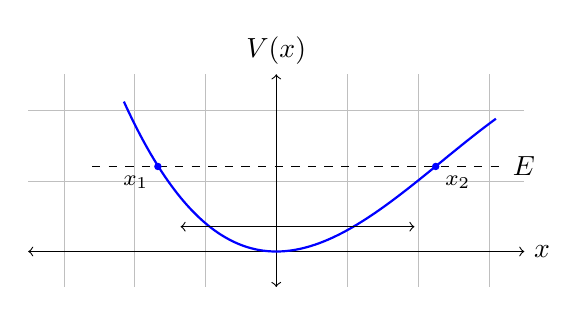
\begin{tikzpicture}[scale=0.9]
	\draw [ultra thin, color=lightgray] (-3.5,-0.5) grid (3.5,2.5);
	\draw [<->] (-3.5, 0) -- (3.5, 0) node [right] {$x$};
	\draw [<->] (0, -0.5) -- (0, 2.5) node [above] {$V(x)$};
	\draw [thick, samples=100, smooth, color=blue, domain=-2.15:3.1] plot (\x, {0.35*\x*\x - 0.05*\x*\x*\x});
	\draw [dashed] (-2.6, 1.2) -- (3.2, 1.2) node [right] {$E$};
	\fill [blue] (-1.67, 1.2) circle (1.5pt);
	\fill [blue] (2.25, 1.2) circle (1.5pt);
	\node at (-1.67, 1.2) [below left] {\footnotesize $x_1$};
	\node at (2.25, 1.2) [below right] {\footnotesize $x_2$};
	\draw [<->] (-1.35, 0.35) -- (1.95, 0.35);
\end{tikzpicture}
\end{center}

Points where the force vanishes are of particular interest.

\begin{definition}[Equilibrium Point]
	A point $x_0$ is an \vocab{equilibrium point} if $V'(x_0) = 0$, so that a particle placed at rest at $x_0$ remains there for all time.
\end{definition}

To understand the behaviour \emph{near} an equilibrium point, we Taylor expand the potential about $x_0$. Using $V'(x_0) = 0$,
$$
V(x) \approx V(x_0) + \frac{1}{2}V''(x_0)(x - x_0)^2 + \cdots,
$$
and so the equation of motion is approximately
$$
m \ddot{x} \approx -V''(x_0) (x - x_0).
$$
There are two cases worth distinguishing.
\begin{enumerate}[label=(\roman*)]
	\item If $V''(x_0) > 0$, so $x_0$ is a local minimum of the potential, then this is exactly the harmonic oscillator equation: the particle oscillates about $x_0$ with angular frequency
	$$
	\omega = \sqrt{\frac{V''(x_0)}{m}}.
	$$
	We call such an equilibrium point \emph{stable}, and these oscillations \emph{small oscillations} about equilibrium.
	\item If $V''(x_0) < 0$, so $x_0$ is a local maximum, then the solutions are $e^{\pm \gamma t}$ with $\gamma = \sqrt{-V''(x_0)/m}$, and a generic small displacement grows exponentially. The equilibrium is \emph{unstable} -- think of a ball balanced on the top of a hill.
\end{enumerate}

\begin{example}[Motion in a Cubic Potential]
	Let's carry out this programme for a particle of mass $m$ in the potential
	$$
	V(x) = m(x^3 - 3x),
	$$
	sketching-first. We have $V'(x) = 3m(x^2 - 1)$, so the equilibria are at $x = \pm 1$, and $V''(x) = 6mx$ tells us that $x = 1$ (where $V = -2m$) is a stable local minimum while $x = -1$ (where $V = 2m$) is an unstable local maximum. The graph falls away to $-\infty$ on the far left.
	\begin{center}
	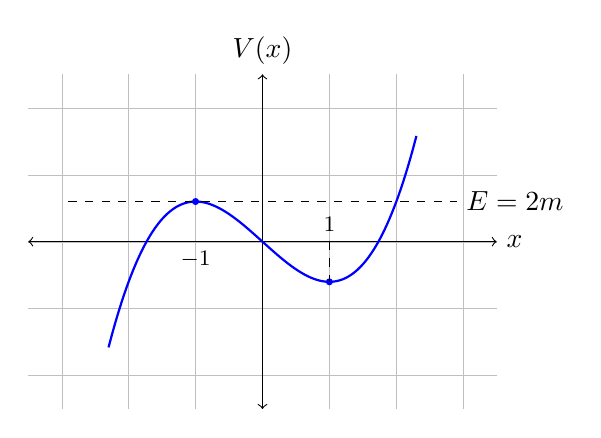
\begin{tikzpicture}[scale=0.85]
		\draw [ultra thin, color=lightgray] (-3.5,-2.5) grid (3.5,2.5);
		\draw [<->] (-3.5, 0) -- (3.5, 0) node [right] {$x$};
		\draw [<->] (0, -2.5) -- (0, 2.5) node [above] {$V(x)$};
		\draw [thick, samples=100, smooth, color=blue, domain=-2.3:2.3] plot (\x, {0.3*\x*\x*\x - 0.9*\x});
		\draw [dashed] (-2.9, 0.6) -- (2.9, 0.6) node [right] {$E = 2m$};
		\fill [blue] (-1, 0.6) circle (1.5pt);
		\fill [blue] (1, -0.6) circle (1.5pt);
		\node at (-1, 0) [below] {\footnotesize $-1$};
		\node at (1, 0) [above] {\footnotesize $1$};
		\draw [dashed] (1, 0) -- (1, -0.6);
	\end{tikzpicture}
	\end{center}
	Now release the particle from rest at various starting points and read off the motion from the graph:
	\begin{enumerate}[label=(\roman*)]
		\item Released near $x = 1$, the particle oscillates in the potential well about the stable equilibrium; for small displacements the angular frequency is $\omega = \sqrt{V''(1)/m} = \sqrt{6}$.
		\item Released anywhere with total energy $E < 2m$ and to the right of the potential hill, the particle remains trapped in the well, oscillating between the two solutions of $V(x) = E$ flanking $x = 1$.
		\item Released with $E > 2m$, the particle clears the hill at $x = -1$ and escapes to $x \to -\infty$, never to return.
		\item The critical case $E = 2m$ is the interesting one: a particle heading leftward towards the hilltop slows down more and more, \emph{approaching} the unstable equilibrium $x = -1$ but never reaching it in finite time (near the top, $\dot{x} \propto (x+1)$, giving exponential approach). The hilltop is reached only `after infinite time'.
	\end{enumerate}
	All of this qualitative information came from a sketch and no integration whatsoever.
\end{example}

\begin{example}[The Pendulum]
	A pendulum consists of a mass $m$ attached to a light rod of length $\ell$, swinging from a fixed pivot.
	\begin{center}
	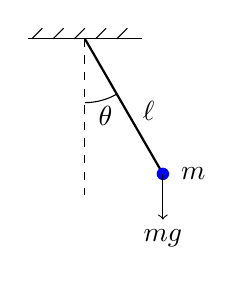
\begin{tikzpicture}[scale=0.9]
		\draw (-0.8, 0) -- (0.8, 0);
		\foreach \x in {-0.75, -0.45, -0.15, 0.15, 0.45} \draw (\x, 0) -- (\x + 0.15, 0.15);
		\draw [dashed] (0, 0) -- (0, -2.2);
		\draw [thick] (0, 0) -- (1.1, -1.905);
		\fill [blue] (1.1, -1.905) circle (2.5pt);
		\node at (1.22, -1.9) [right] {$m$};
		\node at (0.68, -1.02) [right] {$\ell$};
		\draw (0, -0.9) arc (270:300:0.9);
		\node at (0.29, -1.08) {$\theta$};
		\draw [->] (1.1, -1.905) -- (1.1, -2.55) node [below] {$m \vv g$};
	\end{tikzpicture}
	\end{center}
	If $\theta$ is the angle from the downward vertical, the equation of motion is (as can be derived by resolving forces, or by using the energy below)
	$$
	m\ell \ddot{\theta} = -mg \sin \theta.
	$$
	This is of our potential form with generalised coordinate $x = \ell\theta$, with energy
	$$
	E = \frac{1}{2}m\ell^2 \dot{\theta}^2 - mg\ell \cos\theta.
	$$
	The equilibria are $\theta = 0$ (stable) and $\theta = \pi$ (unstable, the pendulum balanced upside-down). Near $\theta = 0$ we have $\sin \theta \approx \theta$, and we recover a harmonic oscillator with angular frequency $\omega = \sqrt{g/\ell}$, so the period of small oscillations is
	$$
	\tau = 2\pi \sqrt{\frac{\ell}{g}},
	$$
	independent of the amplitude and of the mass. For larger swings the period does depend on the amplitude: using conservation of energy, a pendulum released from rest at angle $\theta_0$ has
	$$
	\dot\theta = \pm\sqrt{\frac{2g}{\ell}(\cos\theta - \cos\theta_0)},
	$$
	and separating variables gives the period as an integral,
	$$
	\tau = 4\sqrt{\frac{\ell}{2g}} \int_0^{\theta_0} \frac{\dd\theta}{\sqrt{\cos \theta - \cos \theta_0}},
	$$
	which cannot be evaluated in elementary terms (it is an \emph{elliptic integral}), but which can happily be studied asymptotically or numerically.
\end{example}

\subsection{Potentials in Three Dimensions}

The concept of potentials generalises into three dimensions, but there is some groundwork needed to be done first. We first will need to redefine kinetic energy to make sense in multiple dimensions. This is done naturally with
$$
T = \frac{1}{2} m \dot{\vv x} \cdot \dot{\vv x}.
$$
Differentiating and using Newton's second law, we get $\dot{T} = m \ddot{\vv x} \cdot \dot{\vv x} = \vv F \cdot \dot{\vv x}$, so the kinetic energy changes at a rate given by the component of force along the direction of motion. In particular, a force which is always perpendicular to the velocity does not change the particle's speed.

Now consider a force field $\vv F(\vv x)$, depending only on position.  If the force $\vv F$ acts on a particle, moving it from $\vv x(t_1)$ to $\vv x(t_2)$ along a trajectory $\mathcal{C}$, we define the \emph{work done} $W$ to be
$$
W = \int_\mathcal{C} \vv F \cdot \dd \vv x = \int_{t_1}^{t_2} \vv F \cdot \frac{\dd \vv x}{\dd t} \dd t.
$$
Note that if $\vv F = m \ddot{\vv x}$ (as in there is no change in mass), then integrating the expression for $\dot T$ above shows that the work done is
$$
W = m \int_{t_1}^{t_2} \ddot{\vv x} \cdot \dot{\vv x} \dd t = T(t_2) - T(t_1),
$$
so the work done by the force is the change in kinetic energy of the particle.

In one dimension, every force $F(x)$ had a potential -- we just integrated. In three dimensions this is no longer true: the work done by a general force field can depend on the \emph{path} taken between the endpoints, in which case there is no way to consistently assign a potential energy to positions. The forces for which this does work get a special name.

\begin{definition}[Conservative Force]
	A force field $\vv F(\vv x)$ is \vocab{conservative} if it can be written as
	$$
	\vv F = -\nabla V
	$$
	for some scalar potential $V(\vv x)$, or equivalently\footnote{The equivalence of these conditions (on suitable domains), along with the equivalent statement $\nabla \times \vv F = \vv 0$, is established properly in the `Vector Calculus' course.} if the work done by $\vv F$ along a trajectory depends only on the endpoints of the trajectory.
\end{definition}

\begin{proposition}
	If $\vv F = -\nabla V$, then the total energy
	$$
	E = T + V(\vv x) = \frac{1}{2}m \dot{\vv x} \cdot \dot{\vv x} + V(\vv x)
	$$
	is conserved.
\end{proposition}
\begin{proof}
	We differentiate, using the chain rule $\frac{\dd}{\dd t}V(\vv x(t)) = \nabla V \cdot \dot{\vv x}$:
	\[
	\frac{\dd E}{\dd t} = m \ddot{\vv x}\cdot \dot{\vv x} + \nabla V \cdot \dot{\vv x} = \left(m \ddot{\vv x} - \vv F\right)\cdot \dot{\vv x} = 0. \qedhere
	\]
\end{proof}

Conversely, if a force depending only on position conserves energy for every trajectory, it must be conservative in the above sense. Happily, the fundamental forces of nature that we will meet -- gravity and (static) electromagnetism -- are conservative.

\subsection{Gravity}

Gravity is an example of a conserved force. For a particle of mass $m$, under the influence of gravity from a particle of mass $M$ at the origin, we have the potential energy
$$
V(r) = -\frac{GMm}{r}.
$$
The force of gravity is then given by
$$
\vv F = - \nabla V = -\frac{G Mm}{r^2} \hh r,
$$
with $\hh r$ in the direction of the particle. Note that this force points towards the origin.
It is sometimes convenient to remove the dependence on the mass of the particle $m$, which we do by defining the \emph{gravitational potential} $\phi(r) = -GM/r$, with $V = \phi m$.

If there is many particles say of masses $M_i$ and positions $\vv r_i$, the gravitational potential just adds, with
\begin{align*}
	\phi(\vv r) &= -G \sum_i \frac{M_i}{|\vv r - \vv r_i|} \\
\implies \vv F &= -Gm \sum_i \frac{M_i}{|\vv r - \vv r_i|^3} (\vv r - \vv r_i).
\end{align*}
A remarkable fact (which we will take on trust -- it is a pleasant exercise in vector calculus) is that the external gravitational potential of a spherically symmetric body of total mass $M$ is exactly that of a point mass $M$ at its centre. This is what lets us treat planets and stars as particles when studying orbits.

\begin{example}[Gravity Near the Earth's Surface]
	Consider a particle of mass $m$ at height $z \ll R$ above the surface of the Earth, which has mass $M$ and radius $R$. The potential energy is
	$$
	V = -\frac{GMm}{R + z} = -\frac{GMm}{R}\left(1 - \frac{z}{R} + \cdots\right) \approx \text{const} + mgz,
	$$
	where we define
	$$
	g = \frac{GM}{R^2} \approx \SI{9.8}{\meter\per\second\squared}.
	$$
	So near the surface of the Earth we may use the familiar uniform-gravity potential $V = mgz$, and every particle falls with the same acceleration $g$.
\end{example}

There is a genuinely deep assumption hiding in all of this. The mass appearing in Newton's second law (the \emph{inertial mass}, measuring reluctance to accelerate) and the mass appearing in the law of gravitation (the \emph{gravitational mass}, playing the role of a `gravitational charge') have no a priori reason to be equal -- yet experimentally they agree to extraordinary precision, which is why all bodies fall at the same rate. This equality, the \emph{equivalence principle}, later became the starting point for Einstein's theory of general relativity.

\subsection{Electromagnetism}

If we have time-independent electric and magnetic fields $\vv E$ and $\vv B$, then $\vv E = - \nabla \phi$ for some $\phi(\vv x)$, the \emph{electric potential}. We have conservation of energy for time-independent fields, with the total energy\footnote{Again, this can be checked by differentiating.}
$$
E = \frac{1}{2}m \dot{\vv x} \cdot \dot{\vv x} + q \phi(\vv x). 
$$

Just as objects with mass both feel the effect of and product gravitational force, the same is true of objects with charge. At the origin, a particle of charge $Q$ creates an electric field as
$$
E = - \nabla \left(\frac{Q}{4 \pi \varepsilon_0 r}\right) = \frac{Q}{4 \pi \varepsilon_0} \frac{\hh r}{r^2},
$$
where $r^2 = \vv x \cdot \vv x$. The force between objects of charge $Q$ and $q$ is $\vv F = q \vv E$, or
$$
\vv F = \frac{Qq}{4 \pi \varepsilon_0} \frac{\hh r}{r^2}.
$$
This is the \emph{Coulomb force}, and has the same form as gravity -- an inverse square law -- with one important difference: charges come in both signs, so the Coulomb force can be attractive (unlike charges) or repulsive (like charges).

The magnetic part of the Lorentz force is stranger, since it depends on velocity. Note however that the magnetic force $q\dot{\vv x} \times \vv B$ is always perpendicular to the velocity, so it does no work -- a magnetic field can bend a particle's path, but never change its speed.

\begin{example}[Motion in a Uniform Magnetic Field]
	Consider a particle of charge $q$ and mass $m$ in a uniform magnetic field $\vv B = B \vv e_z$, with no electric field. The equation of motion $m\ddot{\vv x} = q \dot{\vv x} \times \vv B$ has components
	$$
	m \ddot{x} = q B\dot{y} , \quad m \ddot{y} = -qB \dot{x}, \quad m \ddot{z} = 0.
	$$
	The $z$ motion is uniform. For the rest, write $\omega = qB/m$ and combine the first two equations using the complex variable $\zeta = x + iy$:
	$$
	\ddot{\zeta} = \ddot x + i \ddot y = \omega \dot y - i \omega \dot x = -i\omega \dot{\zeta},
	$$
	so $\dot{\zeta} = \dot\zeta_0 e^{-i\omega t}$ and hence $\zeta = \zeta_0 + \frac{i\dot\zeta_0}{\omega}e^{-i \omega t}$. In the $(x, y)$ plane the particle therefore moves in a circle, traversed with constant angular speed
	$$
	\omega = \frac{qB}{m},
	$$
	called the \vocab{gyrofrequency} (or cyclotron frequency). Combined with the uniform drift in $z$, the general trajectory is a helix winding around the magnetic field lines. Note that, as promised, the speed of the particle never changes.
\end{example}

\subsection{Friction}

In many physical scenarios we deal with forces that do not come from potentials. Friction is one such force, and it is a force that is used to approximate the complex relationship between objects in contact.

One common form of friction is \emph{dry friction}, which acts when solid bodies are in contact. If $N$ is the magnitude of the normal reaction force between the surfaces, then the frictional force acts tangentially to the surfaces, opposing relative motion, with magnitude
$$
|\vv F| = \mu N
$$
when the surfaces slide over each other, where $\mu$ is the \emph{coefficient of friction} (which depends on the materials involved). When the surfaces are not sliding, the friction takes whatever magnitude is required to prevent slipping, up to a maximum of roughly $\mu N$. Note that friction opposes relative motion -- it never causes it.

Another common type of friction is \emph{fluid drag}, the resistance felt by a body moving through a fluid. Fluid drag is typically modelled as either
\begin{itemize}
	\item \emph{linear} drag, with $\vv F = - \gamma \vv v$, suitable for small, slow-moving objects in viscous fluids (for a sphere of radius $R$, Stokes' law gives $\gamma = 6\pi \eta R$ where $\eta$ is the fluid's viscosity); or
	\item \emph{quadratic} drag, with $\vv F = - \gamma |\vv v| \vv v$, suitable for larger, fast-moving objects in less viscous fluids such as air, where the resistance comes mostly from the momentum transferred to the fluid pushed out of the way.
\end{itemize}
In either case, the drag force does negative work $\vv F \cdot \vv v < 0$, so the particle continually loses energy to the fluid (where it ends up as heat).

Let's now put several of our forces together in a classic worked example -- a projectile moving under gravity, experiencing linear drag.

\begin{example}[Projectile with Linear Drag]
	A projectile of mass $m$ is launched from the origin with initial velocity $\vv u$, moving under uniform gravity and linear air resistance. The equation of motion is
	$$
	m \frac{\dd \vv v}{\dd t} = m \vv g - \gamma \vv v.
	$$
	This is a linear first order equation for $\vv v$, which we can solve with an integrating factor $e^{\gamma t/m}$:
	$$
	\frac{\dd}{\dd t}\left(e^{\gamma t/m} \vv v\right) = e^{\gamma t/m}\, \vv g \implies \vv v(t) = \frac{m \vv g}{\gamma} + \left(\vv u - \frac{m \vv g}{\gamma}\right)e^{-\gamma t/m}.
	$$
	As $t \to \infty$, the velocity tends to the \vocab{terminal velocity} $\vv v_\infty = m\vv g/\gamma$, in which the drag exactly balances gravity -- and it does so exponentially quickly, on the timescale $m/\gamma$, regardless of the initial conditions.

	Integrating once more gives the trajectory:
	$$
	\vv x(t) = \frac{m \vv g}{\gamma} t + \frac{m}{\gamma}\left(\vv u - \frac{m \vv g}{\gamma}\right)\left(1 - e^{-\gamma t/m}\right).
	$$
	Taking $\vv g = -g \vv e_z$ and $\vv u = (u \cos \theta, 0, u \sin \theta)$, the components read
	$$
	x(t) = \frac{mu\cos\theta}{\gamma}\left(1 - e^{-\gamma t/m}\right), \qquad z(t) = -\frac{mg}{\gamma}t + \frac{m}{\gamma}\left(u \sin\theta + \frac{mg}{\gamma}\right)\left(1 - e^{-\gamma t/m}\right).
	$$
	Two sanity checks are worth performing. First, as $\gamma \to 0$ (expanding the exponentials to second order) we recover the familiar drag-free parabola $x = ut\cos\theta$, $z = ut \sin \theta - \frac{1}{2}gt^2$. Secondly, note that $x$ is bounded: $x < mu\cos\theta/\gamma$ always, so unlike the parabola, the trajectory has a vertical asymptote -- the projectile ends up falling essentially straight down at terminal velocity.
\end{example}

\begin{example}[Falling Raindrop with Quadratic Drag]
	For a raindrop falling vertically under quadratic drag, taking $v$ to be the downward speed,
	$$
	m \frac{\dd v}{\dd t} = mg - \gamma v^2 = \gamma\left(v_\infty^2 - v^2\right), \quad \text{where } v_\infty = \sqrt{\frac{mg}{\gamma}}.
	$$
	Separating variables and using partial fractions,
	$$
	\int \frac{\dd v}{v_\infty^2 - v^2} = \frac{\gamma}{m} t + \text{const} \implies v(t) = v_\infty \tanh\left(\frac{g t}{v_\infty}\right)
	$$
	for a drop released from rest. Again the speed approaches the terminal velocity $v_\infty$, this time with the characteristic $\tanh$ profile.
\end{example}

\section{Dimensional Analysis}

Before going any further with dynamics proper, we pause for a very useful tool. Physical quantities are not pure numbers -- each carries a \emph{dimension}, which is roughly the kind of thing that its units measure. Keeping track of dimensions is a powerful (and almost free) source of information about physical problems.

\subsection{Dimensions of Physical Quantities}

For the problems of dynamics, three basic dimensions suffice:
\begin{itemize}
	\item length, $L$;
	\item mass, $M$;
	\item time, $T$.
\end{itemize}
The dimensions of any other physical quantity $X$ in mechanics, written $[X]$, can then be expressed uniquely as a product of powers of $L$, $M$ and $T$. For example, working directly from the definitions and from equations we know to be true,
\begin{align*}
	[\text{area}] &= L^2, & [\text{velocity}] &= LT^{-1}, & [\text{acceleration}] &= LT^{-2}, \\
	[\text{force}] &= MLT^{-2}, & [\text{energy}] &= ML^2T^{-2}, & [\text{angular momentum}] &= ML^2 T^{-1},
\end{align*}
where, say, the dimensions of force are read off from $F = ma$ and the dimensions of energy from $E = \frac{1}{2}mv^2$. Dimensionful physical constants are treated the same way: from $F = GMm/r^2$ we find $[G] = M^{-1}L^3T^{-2}$.

The key principle is that of \emph{dimensional consistency}: in any meaningful physical equation, both sides must have the same dimensions, and we may only add or subtract terms of equal dimensions. Adding a length to an area is as meaningless as adding a vector to a matrix. Moreover, arguments of functions like $\exp$, $\sin$ or $\log$ must be \emph{dimensionless}: if $x$ had a dimension, the series $e^x = 1 + x + \frac{1}{2}x^2 + \cdots$ would be a sum of terms of different dimensions. (It is a good check on our projectile-with-drag example above that $\gamma t/m$ is dimensionless, since $[\gamma] = [F]/[v] = MT^{-1}$.)

\emph{Units} are conventional reference amounts of dimensional quantities -- in the SI system, the metre, kilogram and second for $L$, $M$ and $T$ respectively. The choice is arbitrary and historical, and no law of physics can depend on it; dimensional consistency is exactly what guarantees that our equations hold in any consistent system of units.

\subsection{Scaling}

These restrictions are not a hindrance -- they are a gift. If we believe that some quantity $Y$ depends only on the quantities $X_1, X_2, X_3$, and the dependence is a power law
$$
Y = C X_1^{p_1} X_2^{p_2} X_3^{p_3}
$$
with $C$ a dimensionless constant, then taking dimensions of both sides gives three linear equations for the three exponents $p_1, p_2, p_3$ (one for each of $L$, $M$, $T$). Provided the dimensions of $X_1, X_2, X_3$ are independent, these determine the exponents uniquely -- so we learn the entire form of the physical law, up to the constant $C$, without solving any dynamics at all.

If there are more than three quantities involved, their dimensions can no longer be independent, and we can form dimensionless combinations $\lambda_1, \lambda_2, \dots$ of the variables. The most general relationship then takes the form
$$
Y = f(\lambda_1, \lambda_2, \dots)\, X_1^{p_1} X_2^{p_2} X_3^{p_3},
$$
where $f$ is an undetermined dimensionless function\footnote{This is a special case of what is formally known as the \emph{Buckingham Pi theorem}.}. Dimensional analysis cannot pin down $f$ -- but knowing the scaling structure is often most of the battle.

\begin{example}[The Simple Pendulum, by Dimensional Analysis]
	Consider again the pendulum: a mass $m$ on a light rod of length $\ell$, released from rest a horizontal distance $d$ from the vertical through the pivot, swinging under gravity $g$. What can the period $\tau$ depend on? Our candidate variables have dimensions
	$$
	[m] = M, \quad [\ell] = L, \quad [g] = LT^{-2}, \quad [d] = L,
	$$
	and $[\tau] = T$. The first three have independent dimensions, and from the fourth we can form the dimensionless group $d/\ell$. So the relationship must be of the form
	$$
	\tau = f\left(\frac{d}{\ell}\right) m^{p_1} \ell^{p_2} g^{p_3},
	$$
	and balancing dimensions,
	$$
	T = M^{p_1} L^{p_2 + p_3} T^{-2p_3} \implies p_1 = 0, \quad p_3 = -\frac{1}{2}, \quad p_2 = \frac{1}{2}.
	$$
	Hence
	$$
	\tau = f\left(\frac{d}{\ell}\right)\sqrt{\frac{\ell}{g}}.
	$$
	Without solving any differential equation, we have learnt that the period is independent of the mass, and scales as $\sqrt{\ell/g}$: if $\ell$ and $d$ are both quadrupled, the period doubles. Comparing with our earlier small-oscillation result $\tau = 2\pi\sqrt{\ell/g}$, we see that $f(x) \to 2\pi$ as $x \to 0$.
\end{example}

\begin{example}[The Speed of Water Waves]
	How fast do waves travel on deep water? Plausibly the wave speed $v$ depends on the wavelength $\Lambda$, the water density $\rho$, and gravity $g$ (which provides the restoring force). These three have independent dimensions, so we look for
	$$
	v = C \Lambda^{p_1} \rho^{p_2} g^{p_3},
	$$
	and balancing dimensions,
	$$
	LT^{-1} = L^{p_1} (ML^{-3})^{p_2} (LT^{-2})^{p_3} \implies p_2 = 0, \quad p_3 = \frac{1}{2}, \quad p_1 = \frac{1}{2}.
	$$
	So
	$$
	v = C\sqrt{g \Lambda}.
	$$
	The density drops out entirely, and long waves travel faster than short ones -- which is why the long, slow swell from a distant storm arrives at the beach before the choppy short waves do. (A full fluid-dynamical calculation gives $C = 1/\sqrt{2\pi}$.)
\end{example}

\begin{example}[Taylor's Estimate of a Blast Energy]
	A famous (and true) story: in 1950, G.\ I.\ Taylor estimated the (then classified) energy yield of the first atomic bomb from declassified photographs of the fireball, using nothing but dimensional analysis. Suppose the radius $R$ of the blast wave at time $t$ after the explosion depends only on $t$, the energy released $E$, and the density $\rho$ of the surrounding air:
	$$
	R = C E^{p_1} \rho^{p_2} t^{p_3}.
	$$
	Balancing dimensions with $[E] = ML^2T^{-2}$ and $[\rho] = ML^{-3}$,
	$$
	L = M^{p_1 + p_2} L^{2p_1 - 3p_2} T^{-2p_1 + p_3} \implies p_1 = \frac{1}{5}, \quad p_2 = -\frac{1}{5}, \quad p_3 = \frac{2}{5}.
	$$
	So
	$$
	R = C\left(\frac{E t^2}{\rho}\right)^{1/5} \implies E \sim \frac{\rho R^5}{t^2},
	$$
	taking the undetermined constant $C$ to be of order $1$. Reading off $R$ at known times $t$ from the photographs gave Taylor an estimate of about $20$ kilotons of TNT -- embarrassingly close to the classified value.
\end{example}

Dimensional analysis is not magic, and it is worth being honest about its limits: it cannot produce dimensionless constants (the $2\pi$ in the pendulum period), it cannot help if we have misidentified which quantities are relevant, and when there are many dimensionless groups it constrains the answer only loosely. But as a first line of attack on any physical problem -- and as an ever-present check on the sanity of our formulae -- it is hard to beat.




\section{Orbits}

We now turn to one of the triumphs of Newtonian mechanics -- the description of the motion of planets, comets, moons and satellites. The key structural feature of all of these problems is that the force always points towards a fixed centre, and we will see that this alone constrains the motion enormously.

\subsection{Central Forces}

If a force is given by a potential $V$, depending only on the distance from the origin, then
$$
\vv F(\vv x) = - \nabla V(|\vv x|) = - \frac{\dd V}{\dd r} \hh r,
$$
where $\hh r = \vv x/|\vv x|$. Such forces are known as \vocab{central forces} -- the force is always parallel to the position vector. Gravity due to a mass fixed at the origin and the Coulomb force due to a fixed charge are the standard examples.

\subsection{Angular Momentum}

An important result when dealing with central forces is the existence of another conserved quantity, \emph{angular momentum}.

\begin{definition}[Angular Momentum]
	The \vocab{angular momentum} of a particle about the origin is
	$$
	\vv L = \vv x \times \vv p = m \vv x \times \dot{\vv x}.
	$$
\end{definition}

Note that, unlike momentum, angular momentum depends on the choice of origin -- it measures something like `the amount of rotation about the origin'. Let's see how it changes in time. With a general force $\vv F$,
$$
\frac{\dd \vv L}{\dd t} = m\dot{\vv x} \times \dot{\vv x} + m \vv x \times \ddot{\vv x} = \vv x \times \vv F = \vv \tau,
$$
a quantity named \emph{torque} (about the origin). This is the rotational analogue of Newton's second law: torque is the rate of change of angular momentum.

\begin{proposition}
	For motion in a central force, angular momentum is conserved.
\end{proposition}
\begin{proof}
	If the force is central, then $\vv F \parallel \vv x$, so $\vv \tau = \vv x \times \vv F = \vv 0$, and thus $\dot{\vv L} = \vv 0$.
\end{proof}

This conservation law has an immediate geometric consequence. Since $\vv L = m \vv x \times \dot{\vv x}$ is a constant vector and $\vv x \cdot \vv L = 0$ always, the position vector is confined to the plane through the origin perpendicular to $\vv L$.\footnote{If $\vv L = \vv 0$, then $\vv x$ and $\dot{\vv x}$ are always parallel, and the motion takes place on a straight line through the origin -- which is certainly also planar.} So \emph{motion in a central force is planar}, and a problem that started in three dimensions is now a problem in two. We will shortly reduce it to one.

\subsection{Polar Coordinates in the Plane}

Since the motion is planar, it makes sense to use coordinates adapted to the geometry: plane polar coordinates $(r, \theta)$, with $x = r \cos\theta$ and $y = r \sin \theta$. We use the orthonormal basis vectors
$$
\hh r = \begin{pmatrix} \cos \theta \\ \sin\theta\end{pmatrix}, \quad \hh \theta = \begin{pmatrix} -\sin\theta \\ \cos\theta \end{pmatrix},
$$
pointing in the directions of increasing $r$ and $\theta$ respectively.
\begin{center}
\begin{tikzpicture}[scale=1.0]
	\draw [->] (-0.4, 0) -- (3.2, 0) node [right] {$x$};
	\draw [->] (0, -0.4) -- (0, 2.6) node [above] {$y$};
	\draw (0, 0) -- (1.8, 1.35) node [pos = 0.5, above left = -2pt] {$r$};
	\fill (1.8, 1.35) circle (1.5pt);
	\draw [->, thick, color=blue] (1.8, 1.35) -- (2.44, 1.83) node [right] {$\hh r$};
	\draw [->, thick, color=blue] (1.8, 1.35) -- (1.32, 1.99) node [above] {$\hh \theta$};
	\draw (0.7, 0) arc (0:36.87:0.7);
	\node at (0.92, 0.26) {$\theta$};
\end{tikzpicture}
\end{center}
The subtlety, and the entire content of what follows, is that these basis vectors \emph{depend on the position of the particle}, so they change as the particle moves. Differentiating the expressions above with respect to $\theta$,
$$
\frac{\dd \hh r}{\dd \theta} = \hh \theta, \quad \frac{\dd \hh \theta}{\dd\theta} = - \hh r.
$$

\begin{proposition}[Velocity and Acceleration in Polar Coordinates]
	For a particle with position $\vv x = r \hh r$,
	\begin{align*}
		\dot{\vv x} &= \dot{r} \hh r + r \dot{\theta} \hh \theta, \\
		\ddot{\vv x} &= (\ddot{r} - r \dot{\theta}^2)\hh r + (r \ddot{\theta} + 2 \dot{r}\dot{\theta}) \hh \theta.
	\end{align*}
\end{proposition}
\begin{proof}
	By the chain rule, $\dot{\hh r} = \dot\theta \, \hh \theta$ and $\dot{\hh \theta} = -\dot\theta\, \hh r$. So differentiating $\vv x = r \hh r$,
	$$
	\dot{\vv x} = \dot{r}\hh r + r \dot{\hh r} = \dot{r} \hh r + r \dot{\theta} \hh \theta,
	$$
	and differentiating again,
	\[
	\ddot{\vv x} = \ddot{r} \hh r + \dot{r}\dot{\theta} \hh\theta + \dot{r}\dot\theta \hh \theta + r \ddot{\theta}\hh\theta - r \dot{\theta}^2 \hh r = (\ddot{r} - r \dot\theta^2)\hh r + (r \ddot\theta + 2 \dot{r}\dot\theta)\hh\theta. \qedhere
	\]
\end{proof}

The term $-r\dot\theta^2 \hh r$ should be familiar: for a particle moving on a \emph{circle} of constant radius $r$ with angular speed $\omega = \dot\theta$, the acceleration is $-r\omega^2 \hh r$, of magnitude $r\omega^2 = v^2/r$ directed towards the centre -- the \emph{centripetal acceleration}. Some force must supply this if a particle is to move in a circle.

\begin{example}[Circular Orbit Speed]
	For a satellite in a circular orbit of radius $r$ about the Earth, gravity supplies the centripetal force:
	$$
	\frac{mv^2}{r} = \frac{GMm}{r^2} \implies v = \sqrt{\frac{GM}{r}}.
	$$
	The period is then $\tau = 2\pi r / v = 2\pi r^{3/2}/\sqrt{GM}$ -- a first glimpse of Kepler's third law, to which we will return.
\end{example}

\subsection{Reduction to One Dimension}

Suppose we had a potential $V(r)$, with $\vv F = - \nabla V = - \dd V/\dd r \, \hh r$. Newton's second law in the plane with plane polar coordinates $(r, \theta)$ is (for constant mass)
\begin{align*}
	m \ddot{\vv x} &= - \frac{\dd V}{\dd r} \hh r \\
\implies m (\ddot{r} - r \dot{\theta}^2) \hh r + m (r \ddot{\theta} + 2 \dot{r} \dot{\theta}) \hh \theta &= -\frac{\dd V}{\dd r} \hh r.
\end{align*}
Then since the components are orthogonal, we can then obtain two separate equations. The first (taking the $\hh \theta$ component) is
\begin{align*}
	r \ddot{\theta} + 2 \dot{r} \dot{\theta} = 0 \implies \frac{1}{r} \frac{\dd}{\dd t}(r^2 \dot{\theta}) = 0.
\end{align*}
This is not a surprise but a consistency check: the angular momentum of the system is $\vv L = \vv x \times m \dot{\vv x} = m r^2 \dot{\theta} (\hh r \times \hh \theta)$, and thus $|\vv L| = m r^2 \dot{\theta} = m \ell$, where $\ell = r^2 \dot\theta$ is the angular momentum per unit mass. So this equation just says that angular momentum is conserved, which we already knew.

The other component then gives us the equation
$$
m(\ddot{r} - r \dot{\theta}^2) = - \frac{\dd V}{\dd r} \implies m \ddot{r} = -\frac{\dd V}{\dd r} + m r \dot{\theta}^2 = - \frac{\dd V}{\dd r} + \frac{m\ell^2}{r^3},
$$
where in the last step we eliminated $\dot\theta$ using $\dot\theta = \ell/r^2$. Thus we have reduced our three dimensional problem of a central force into a one dimensional problem involving the radial component only -- the price being an extra, angular-momentum-dependent term in the force.

\subsection{The Effective Potential}

Using our reduced problem, we can `forget' about the $\theta$ component, and consider a one dimensional system, under the influence of the \emph{effective potential}
$$
V_{\text{eff}}(r) = V(r) + \frac{m \ell^2}{2r^2}.
$$
The rightmost term is the \emph{angular momentum barrier}, and it stops the particle from getting too close to the origin: as $r \to 0$ it blows up like $1/r^2$, which (for potentials less singular than this, such as gravity) dominates and repels the particle.

We can even use this viewpoint in energy conservation, as
$$
E = \frac{1}{2}m \dot{\vv x} \cdot \dot{\vv x} + V(r) = \frac{1}{2}m \dot{r}^2 + V_{\text{eff}}(r),
$$
using $|\dot{\vv x}|^2 = \dot{r}^2 + r^2 \dot\theta^2$ and $\dot\theta = \ell/r^2$. So all our one dimensional technology -- sketching the potential, classifying allowed regions by energy, finding equilibria -- applies directly to the radial motion.

\begin{example}[Orbits in an Inverse Square Law Potential]
	For gravity, $V(r) = -GMm/r$, the effective potential
	$$
	V_{\text{eff}}(r) = -\frac{GMm}{r} + \frac{m\ell^2}{2r^2}
	$$
	tends to $+\infty$ as $r \to 0$ (the angular momentum barrier wins), and tends to $0^-$ as $r \to \infty$, with a single minimum in between at $r_* = \ell^2/GM$.
	\begin{center}
	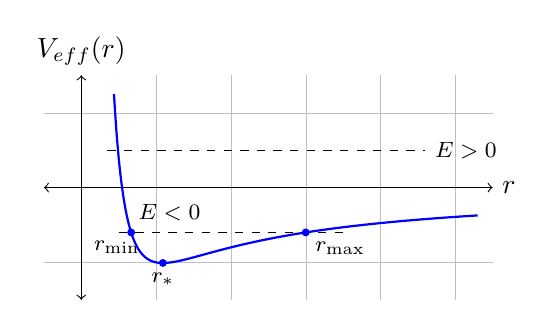
\begin{tikzpicture}[scale=0.95]
		\draw [ultra thin, color=lightgray] (-0.5,-1.5) grid (5.5,1.5);
		\draw [<->] (-0.5, 0) -- (5.5, 0) node [right] {$r$};
		\draw [<->] (0, -1.5) -- (0, 1.5) node [above] {$V_{\text{eff}}(r)$};
		\draw [thick, samples=150, smooth, color=blue, domain=0.437:5.3] plot (\x, {1.2/(\x*\x) - 2.2/\x});
		\draw [dashed] (0.35, 0.5) -- (4.6, 0.5) node [right] {\footnotesize $E > 0$};
		\draw [dashed] (0.5, -0.6) -- (3.5, -0.6);
		\node at (1.18, -0.33) {\footnotesize $E < 0$};
		\fill [blue] (0.667, -0.6) circle (1.5pt);
		\fill [blue] (3, -0.6) circle (1.5pt);
		\node at (0.04, -0.8) [right] {\footnotesize $r_{\min}$};
		\node at (3, -0.6) [below right] {\footnotesize $r_{\max}$};
		\fill [blue] (1.091, -1.008) circle (1.5pt);
		\node at (1.091, -1.008) [below] {\footnotesize $r_*$};
	\end{tikzpicture}
	\end{center}
	Reading off the qualitative motion from the graph:
	\begin{enumerate}[label=(\roman*)]
		\item If $E = V_{\text{eff}}(r_*)$, then $r = r_*$ is constant, and the orbit is a \emph{circle}.
		\item If $V_{\text{eff}}(r_*) < E < 0$, the radius oscillates between two values $r_{\min} \leq r \leq r_{\max}$ (the \emph{perihelion} and \emph{aphelion}) -- the orbit is bounded.
		\item If $E \geq 0$, the particle can escape to $r \to \infty$ -- the orbit is unbounded, and the particle approaches, swings past, and leaves, never to return.
	\end{enumerate}
	We will see shortly that the bounded orbits are precisely ellipses, and the unbounded ones hyperbolae (or, in the marginal case $E = 0$, parabolae).
\end{example}

\begin{example}[Finding the Turning Points]
	The perihelion and aphelion distances can be computed directly from the conserved quantities. At a turning point of the radial motion, $\dot{r} = 0$, so $E = V_{\text{eff}}(r)$:
	$$
	E = -\frac{GMm}{r} + \frac{m\ell^2}{2r^2} \implies E r^2 + GMm\, r - \frac{m\ell^2}{2} = 0,
	$$
	a quadratic in $r$. For bound orbits ($E < 0$) it has two positive roots, $r_{\min}$ and $r_{\max}$, and by the standard formulae for the sum and product of roots,
	$$
	r_{\min} + r_{\max} = -\frac{GMm}{E} \quad (= 2a), \qquad r_{\min}\, r_{\max} = -\frac{m \ell^2}{2E} \quad (= b^2),
	$$
	which the reader may enjoy checking against the geometry of the ellipse. For $E \geq 0$ there is a single positive root -- the distance of closest approach of an unbound trajectory.
\end{example}

\subsection{Stability of Circular Orbits}

A circular orbit at radius $r_*$ exists whenever $V_{\text{eff}}'(r_*) = 0$, and just as for one dimensional potentials, the orbit is \emph{stable} (small perturbations of the radius oscillate rather than grow) precisely when $r_*$ is a minimum of the effective potential, that is when $V_{\text{eff}}''(r_*) > 0$. In that case a slightly perturbed orbit has radius oscillating about $r_*$ with angular frequency $\omega_r$ given by $m\omega_r^2 = V_{\text{eff}}''(r_*)$.

\begin{example}[Stability for Power Law Forces]
	Suppose the force is attractive with $F(r) = -mk/r^n$ for some $n$, so $V(r) = -\frac{mk}{(n-1)r^{n - 1}}$ for $n \neq 1$. Then
	$$
	V_{\text{eff}}(r) = -\frac{mk}{(n - 1) r^{n-1}} + \frac{m \ell^2}{2 r^2},
	$$
	and circular orbits satisfy $V'_{\text{eff}}(r_*) = 0$, giving $\ell^2 = k r_*^{3 - n}$. Computing the second derivative and substituting this in,
	$$
	V_{\text{eff}}''(r_*) = -\frac{nmk}{r_*^{n +1}} + \frac{3m\ell^2}{r_*^4} = \frac{mk}{r_*^{n + 1}}\left(3 - n\right).
	$$
	So circular orbits are stable if and only if $n < 3$. In particular the inverse square law $n = 2$ gives stable circular orbits (reassuring, given that we live on a planet in a nearly circular orbit), while an inverse cube force $n = 3$ or stronger cannot support stable circles -- a slight nudge sends the particle spiralling inwards or outwards.
\end{example}

\subsection{Escape Velocity}

Consider a projectile launched from the surface of a planet of mass $M$ and radius $R$. Ignoring air resistance, when can it escape the planet's gravity entirely? By conservation of energy,
$$
E = \frac{1}{2}mv^2 - \frac{GMm}{r},
$$
and (as we saw from the effective potential) the projectile can reach $r \to \infty$ precisely when $E \geq 0$. Launching from $r = R$, this requires
$$
v \geq v_{\text{esc}} = \sqrt{\frac{2GM}{R}},
$$
the \vocab{escape velocity} of the planet. For the Earth, $v_{\text{esc}} \approx \SI{11.2}{\kilo\meter\per\second}$. Note that $v_{\text{esc}}$ is independent of the mass of the projectile, and (perhaps surprisingly) of the direction of launch: energy conservation cares only about speed. A particle launched at exactly $v_{\text{esc}}$ reaches infinity with nothing to spare, arriving with zero speed.

\subsection{The $u(\theta)$ Equation}

We now want the \emph{shape} of a general orbit, that is, $r$ as a function of $\theta$ rather than of $t$. It turns out that the substitution $u = 1/r$ just seems to work really well when dealing with the system we have set up. Using the chain rule with $\dot\theta = \ell u^2$, we have
\begin{align*}
	\dot{r} &= \frac{\dd r}{\dd \theta} \dot{\theta} = \frac{\dd r}{\dd\theta} \frac{\ell}{r^2} = -\ell \frac{\dd u}{\dd \theta}, \\
	\ddot{r} &= \frac{\dd}{\dd t}\left(- \ell \frac{\dd u}{\dd\theta}\right) = -\ell \frac{\dd^2 u}{\dd\theta^2}\dot{\theta} = -\ell^2 u^2 \frac{\dd^2 u}{\dd \theta^2}.
\end{align*}
Then our equation of motion goes from $m \ddot{r} - m\ell^2/r^3 = F(r)$ to \emph{Binet's equation}:
$$
-m\ell^2 u^2 \left(\frac{\dd^2 u }{\dd \theta^2} + u\right) = F\left(\frac{1}{u}\right).
$$
This is generally still nonlinear -- but for inverse square laws (such as gravity), where $F(1/u) \propto u^2$, the factor of $u^2$ on the left cancels, and it becomes a \emph{linear} equation, one we know exactly how to solve. After it is solved, we can get back the time dependence with $\dot{\theta} = \ell u^2$.

\subsection{The Kepler Problem}

Binet's equation can be used to find the shapes of orbits under an inverse square law. Let
$$
V(r) = -\frac{mk}{r}, \quad F(r) = -\frac{mk}{r^2},
$$
where $k = GM$ for gravity due to a mass $M$ fixed at the origin. Then Binet's equation is
$$
\frac{\dd^2 u}{\dd \theta^2} + u = \frac{k}{\ell^2}.
$$
This is the harmonic oscillator equation (in the variable $\theta$!) with a constant forcing term, so the general solution is
$$
u = \frac{k}{\ell^2} + A \cos(\theta - \theta_0).
$$
Taking $\theta_0 = 0$ (which we can arrange by rotating our coordinates) and $A \geq 0$, we conclude that for a planet in orbit about the origin, the shape of the orbit is given by
$$
r = \frac{p}{1 + e \cos \theta},
$$
with $p = \ell^2/k$ and $e = A \ell^2/k \geq 0$. This is the polar-coordinate equation of a \emph{conic section} with a focus at the origin, where $e$ is the \vocab{eccentricity}. Notice that $r$ is minimised at $\theta = 0$ (the closest approach, or \emph{perihelion} for orbits about the Sun) and, when the orbit is bounded, maximised at $\theta = \pi$ (\emph{aphelion}). The nature of the conic depends on the eccentricity:
\begin{enumerate}[label=(\roman*)]
	\item If $e = 0$ then $r = p$ is constant, and the orbit is a \emph{circle}.
	\item If $0 < e < 1$, the denominator is always positive, so $r$ is bounded with $\frac{p}{1 + e} \leq r \leq \frac{p}{1 - e}$, and the orbit is an \emph{ellipse} with the origin at one focus. In Cartesian coordinates centred appropriately, it has semi-major and semi-minor axes
	$$
	a = \frac{p}{1 - e^2}, \quad b = \frac{p}{\sqrt{1 - e^2}}.
	$$
	\item If $e = 1$, then $r \to \infty$ as $\theta \to \pm \pi$: the orbit is an unbounded \emph{parabola}.
	\item If $e > 1$, then $r \to \infty$ as $\theta \to \pm \alpha$ where $\alpha = \cos^{-1}(1/e) \in (\pi/2, \pi)$: the orbit is one branch of a \emph{hyperbola}, with asymptotes at angles $\pm\alpha$.
\end{enumerate}

The bounded case is the one Kepler cared about -- an ellipse with the attracting body at a focus:

\begin{center}
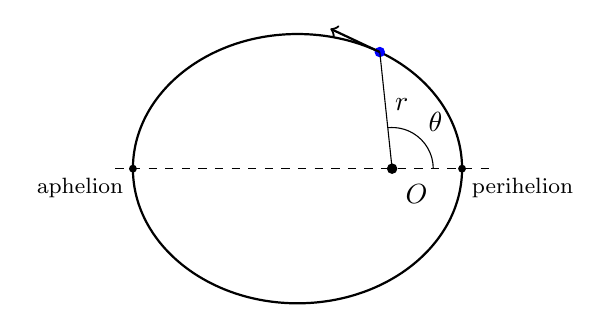
\begin{tikzpicture}[scale=0.95]
	\draw [dashed] (-3.7, 0) -- (1.3, 0);
	\draw [thick] (-1.265, 0) ellipse (2.2 and 1.8);
	\fill (0, 0) circle (2pt);
	\node at (0.05, -0.08) [below right] {$O$};
	\fill [blue] (-0.165, 1.559) circle (2pt);
	\draw (0, 0) -- (-0.165, 1.559) node [pos = 0.55, right] {$r$};
	\draw [->, thick] (-0.165, 1.559) -- (-0.825, 1.87);
	\draw (0.55, 0) arc (0:96:0.55);
	\node at (0.58, 0.62) {$\theta$};
	\fill (0.935, 0) circle (1.5pt);
	\node at (0.935, 0) [below right] {\footnotesize perihelion};
	\fill (-3.465, 0) circle (1.5pt);
	\node at (-3.465, 0) [below left] {\footnotesize aphelion};
\end{tikzpicture}
\end{center}

\begin{example}[Determining an Orbit from Initial Conditions]
	A satellite is at distance $r_0$ from the Earth's centre, moving with speed $v_0$ \emph{perpendicular} to its position vector. What orbit does it follow? Since $\dot{\vv x} \perp \vv x$, the angular momentum per unit mass is $\ell = r_0 v_0$, and this point is an apse of the orbit (a maximum or minimum of $r$), so it lies at $\theta = 0$ or $\theta = \pi$ in our standard form. Comparing $r_0$ with the orbit equation at $\theta = 0$,
	$$
	r_0 = \frac{p}{1 + e} = \frac{r_0^2 v_0^2}{GM(1 + e)} \implies e = \frac{r_0 v_0^2}{GM} - 1.
	$$
	Reading off the cases:
	\begin{enumerate}[label=(\roman*)]
		\item If $v_0^2 = GM/r_0$, then $e = 0$ -- the circular orbit speed we found before.
		\item If $GM/r_0 < v_0^2 < 2GM/r_0$, then $0 < e < 1$: an ellipse with the launch point as perihelion.
		\item If $v_0^2 < GM/r_0$, the formula gives $e < 0$, which just means the launch point is the \emph{aphelion} instead (replace $\theta \mapsto \theta + \pi$): the satellite falls inwards on an ellipse.
		\item If $v_0^2 \geq 2GM/r_0$, then $e \geq 1$ and the satellite escapes on a parabola or hyperbola -- and indeed $v_0 = \sqrt{2GM/r_0}$ is precisely the escape velocity from radius $r_0$ that we found earlier.
	\end{enumerate}
\end{example}

\subsection{Energy and Eccentricity}

Which orbit we get is determined by the energy. Evaluating the conserved energy at perihelion (where $\dot{r} = 0$, $r = p/(1 + e)$ and so $\dot{\vv x} = r\dot\theta \hh\theta$ has magnitude $\ell/r$),
$$
E = \frac{1}{2}\frac{m \ell^2}{r^2} - \frac{mk}{r}\bigg|_{r = p/(1+e)} = \frac{mk^2}{2\ell^2}\left(e^2 - 1\right).
$$
So the classification by eccentricity is exactly the classification by energy that we sketched using the effective potential:
\begin{align*}
	e < 1 &\iff E < 0 && \text{(ellipse)}, \\
	e = 1 &\iff E = 0 && \text{(parabola)}, \\
	e > 1 &\iff E > 0 && \text{(hyperbola)}.
\end{align*}
Bound orbits are precisely those with negative total energy -- the particle does not have enough kinetic energy to climb out of the potential well.

For an elliptical orbit there is a particularly clean way to package the energy. Using $\ell^2 = pk$ and $p = a(1 - e^2)$,
$$
E = \frac{mk^2(e^2 - 1)}{2\ell^2} = \frac{mk^2 (e^2 - 1)}{2 a (1 - e^2)k} = -\frac{mk}{2a},
$$
so the energy of an orbit depends only on its \emph{semi-major axis}, not on its eccentricity -- a circle of radius $a$ and a wildly elongated ellipse of semi-major axis $a$ have exactly the same energy. Writing out $E = \frac{1}{2}mv^2 - mk/r$ and rearranging gives the handy \emph{vis-viva equation},
$$
v^2 = GM\left(\frac{2}{r} - \frac{1}{a}\right),
$$
which gives the speed at any point of the orbit. Sanity checks: for a circle ($r = a$) it reduces to $v^2 = GM/r$, and letting $a \to \infty$ (the parabolic, marginally-escaping orbit) recovers $v^2 = 2GM/r$, the escape velocity.

\subsection{Kepler's Laws}

Long before Newton, Kepler had extracted three empirical laws of planetary motion from Tycho Brahe's astronomical observations.

\begin{law}[Kepler's Laws of Planetary Motion]
	\begin{enumerate}
		\item The orbit of a planet is an ellipse, with the Sun at one focus.
		\item The line between the planet and the Sun sweeps out equal areas in equal times.
		\item The square of the orbital period is proportional to the cube of the semi-major axis, $\tau^2 \propto a^3$.
	\end{enumerate}
\end{law}

Newton's great achievement was to show that all three follow from his laws of motion together with the inverse square law of gravitation -- and we have now assembled everything needed to check this ourselves.

The first law follows from our discussion of the Kepler problem: bounded orbits under an inverse square law are ellipses with a focus at the origin.

The second law is just conservation of angular momentum in geometric clothing, and in fact holds for \emph{any} central force. When the position vector sweeps through a small angle $\dd\theta$, the area swept out is that of a thin triangle, $\dd A = \frac{1}{2}r \cdot r \dd\theta$, so
$$
\frac{\dd A}{\dd t} = \frac{1}{2}r^2 \dot{\theta} = \frac{\ell}{2},
$$
which is constant. A planet therefore moves fastest at perihelion and slowest at aphelion.

\begin{example}
	Conservation of angular momentum relates the extreme speeds directly: at perihelion and aphelion the velocity is purely tangential, so $\ell = r_{\min}v_{\max} = r_{\max}v_{\min}$, giving
	$$
	\frac{v_{\max}}{v_{\min}} = \frac{r_{\max}}{r_{\min}} = \frac{1 + e}{1 - e}.
	$$
	The Earth's orbital eccentricity is a modest $e \approx 0.017$, so its speed varies by only about $3.4\%$ over the year (roughly $30.3$ versus $\SI{29.3}{\kilo\meter\per\second}$). Halley's comet, with $e \approx 0.97$, moves about $66$ times faster at perihelion than at aphelion -- it spends decades dawdling in the outer solar system and mere months whipping around the Sun.
\end{example}

For the third law, integrate the second law over a full orbit: the area of an ellipse is $A = \pi a b$, so
$$
\pi a b = \frac{\ell}{2} \tau.
$$
Now using $b^2 = a^2 (1 - e^2)$ and $\ell^2 = pk = a(1 - e^2)k$,
$$
\tau^2 = \frac{4 \pi^2 a^2 b^2}{\ell^2} = \frac{4\pi^2 a^4 (1 - e^2)}{a(1-e^2)k} = \frac{4 \pi^2}{GM} a^3,
$$
recalling that $k = GM$. So $\tau^2 \propto a^3$, with a constant of proportionality depending only on the mass of the Sun -- which is why the same law holds for every planet in the solar system.

\begin{example}[Geostationary Orbit]
	At what radius does a satellite orbit the Earth once per day, so as to hover over a fixed point on the equator? Rearranging the third law (for a circular orbit, $a = r$),
	$$
	r = \left(\frac{GM \tau^2}{4\pi^2}\right)^{1/3},
	$$
	and inserting $GM \approx \SI{4.0e14}{\meter\cubed\per\second\squared}$ for the Earth and $\tau = \SI{86400}{\second}$ gives $r \approx \SI{4.2e7}{\meter}$, i.e.\ about $\SI{42000}{\kilo\meter}$ from the Earth's centre, or some $\SI{36000}{\kilo\meter}$ above the surface. This is where communications and weather satellites live.
\end{example}

\begin{example}[Halley's Comet]
	The third law works just as well in reverse. Halley's comet returns every $76$ years; measuring in years and astronomical units (in which the Earth's orbit has $\tau = 1$ and $a = 1$, conveniently normalising the constant of proportionality), its semi-major axis is
	$$
	a = \tau^{2/3} = 76^{2/3} \approx 17.9 \text{ AU}.
	$$
	Since the comet's orbit is highly eccentric ($e \approx 0.97$), its distances of closest and furthest approach are $a(1 - e) \approx 0.6$ AU (inside Venus's orbit) and $a(1 + e) \approx 35$ AU (out past Neptune) -- all deduced from its period and one observation of its perihelion.
\end{example}

\subsection{Rutherford Scattering}

Finally, let's consider what happens when the inverse square force is \emph{repulsive}, so
$$
V(r) = +\frac{mk}{r}, \quad F(r) = +\frac{mk}{r^2}, \quad k > 0.
$$
The classic physical setting is Rutherford's famous experiment: alpha particles (charge $q$) fired at gold atoms are repelled by the nucleus (charge $Q$), with $k = Qq/4\pi\varepsilon_0 m > 0$ by the Coulomb force law.

Binet's equation now reads $u'' + u = -k/\ell^2$, with general solution
$$
u = -\frac{k}{\ell^2} + A \cos(\theta - \theta_0),
$$
and taking $\theta_0 = 0$, $A \geq 0$ as usual we get
$$
r = \frac{p}{e \cos \theta - 1}, \quad p = \frac{\ell^2}{k}, \quad e = \frac{A\ell^2}{k}.
$$
For $r$ to be positive we need $e > 1$: \emph{every} orbit in a repulsive inverse square force is a hyperbola (which makes sense -- there can be no bound orbits when the force pushes you away). The particle comes in from infinity, reaches a closest approach at $\theta = 0$, and escapes to infinity again, with $r \to \infty$ as $\theta \to \pm \alpha$ where $\alpha = \cos^{-1}(1/e)$. This time the trajectory is the branch of the hyperbola on the \emph{far side} from the focus, curving away from the origin.

\begin{center}
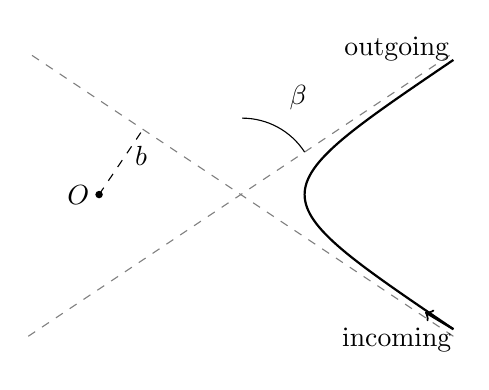
\begin{tikzpicture}[scale=0.9]
	\draw [gray, dashed] (-3, -2) -- (3, 2);
	\draw [gray, dashed] (3, -2) -- (-3, 2);
	\draw [thick] (3, -1.9) .. controls (0.2, 0) .. (3, 1.9);
	\draw [->, thick] (3, -1.9) -- (2.6, -1.66);
	\fill (-2, 0) circle (1.5pt);
	\node at (-2, 0) [left] {$O$};
	\draw [dashed] (-2, 0) -- (-1.38, 0.92) node [pos = 0.6, right] {$b$};
	\draw (0.9, 0.6) arc (33:90:1.05);
	\node at (0.55, 1.05) [above right] {$\beta$};
	\node at (2.2, -1.75) [below] {incoming};
	\node at (2.2, 1.75) [above] {outgoing};
\end{tikzpicture}
\end{center}

The interesting physical question is: by what angle is the particle deflected? Characterise the incoming trajectory by its speed $v$ at infinity, and its \vocab{impact parameter} $b$ -- the perpendicular distance between the incoming asymptote and the origin. Evaluating the conserved quantities far away, the angular momentum per unit mass is $\ell = bv$.

The two asymptotes make angles $\pm \alpha$ with the axis of the hyperbola, so the total \emph{scattering angle} (between the incoming and outgoing directions) is $\beta = \pi - 2\alpha$. Then
$$
\frac{1}{e} = \cos \alpha = \cos\left(\frac{\pi}{2} - \frac{\beta}{2}\right) = \sin \frac{\beta}{2}.
$$
A little algebra with the geometry of the hyperbola shows that the impact parameter is $b = p/\sqrt{e^2 - 1}$, so
$$
b = \frac{\ell^2}{k}\frac{1}{\sqrt{e^2 - 1}} = \frac{(bv)^2}{k} \tan \frac{\beta}{2},
$$
and rearranging,
$$
\beta = 2 \tan^{-1}\left(\frac{k}{b v^2}\right).
$$
Small impact parameters $b \ll k/v^2$ (nearly head-on collisions) give scattering angles approaching $\pi$ -- the particle bounces almost straight back. It was precisely the observation of such large-angle scattering of alpha particles that led Rutherford to conclude that an atom's positive charge is concentrated in a tiny nucleus, rather than being smeared throughout the atom: as he put it, ``it was almost as incredible as if you fired a 15-inch shell at a piece of tissue paper and it came back and hit you.''
\section{Rotating Frames} \label{sec:rotating}

Newton's laws hold in inertial frames -- but many frames we care about are not inertial. The most important example is right beneath our feet: the Earth rotates once a day, so a laboratory fixed to its surface is a rotating frame. In this section we work out what Newton's second law looks like to an observer in a rotating frame, and find that they can continue to use it, provided they are willing to admit some additional `fictitious' forces into their bookkeeping.

\subsection{Motion in Rotating Frames}

Suppose that $\FF$ is an inertial frame, and $\FF'$ is rotating about the $z$ axis with angular velocity $\vv \omega = \omega \vv e_z$ with respect to $\FF$.

Suppose we have basis vectors $\{\vv e_i\}$ and $\{\vv e_i'\}$ in $\FF$ and $\FF'$ respectively. If a particle is at rest in $\FF'$, then in $\FF$ its velocity is given by
	$$
	\left(\frac{\dd \vv r}{\dd t}\right)_{\FF} = \vv \omega \times \vv r.
	$$
	Of course, this also applies to the basis vectors in $\FF'$, with
	$$
	\left(\frac{\dd \vv e_i'}{\dd t}\right)_{\FF} =\vv \omega \times \vv e_i'.
	$$

	Now for some vector $\vv a$, we can write it in the $\{\vv e_i'\}$ basis as
	$$
\vv a = \sum_i a_i'(t) \vv e_i'.
$$
In the frame $\FF'$, the basis vectors $\vv e_i'$ are constant, and thus the derivative of $\vv a$ is given by
$$
\left(\frac{\dd \vv a}{\dd t}\right)_{\FF'} = \sum_i \frac{\dd a_i'(t)}{\dd t} \vv{e}_i'.
$$
In the frame $\FF$ however, the basis vectors $\{\vv e_i'\}$ are not constant, and we have
$$
\left(\frac{\dd \vv a}{\dd t}\right)_{\FF} = \sum_i \frac{\dd a_i'(t)}{\dd t} \vv{e}_i' + \sum_i a_i'(t) \vv \omega \times \vv e_i' = \left(\frac{\dd \vv a}{\dd t}\right)_{\FF'} +\vv \omega \times \vv a
$$

\subsection{Change of Frame Operator}

Let $\FF$ be an inertial frame, and $\FF'$ be rotating relative to $\FF$ with angular velocity $\vv \omega$.
Then we have
$$
\left(\frac{\dd}{\dd t}\right)_{\FF} = \left(\frac{\dd}{\dd t}\right)_{\FF'} +\vv \omega \times 
$$

\subsection{Velocity and Acceleration}

Using the change of frame operator, we can see that
$$
\left(\frac{\dd \vv r}{\dd t}\right)_{\FF} = \left(\frac{\dd \vv r}{\dd t}\right)_{\FF'} +\vv \omega \times \vv r,
$$
and applying the operator again (and noting that $\dot{\vv \omega}$ is the same in both frames), we have
$$
\left(\frac{\dd^2 \vv r}{\dd t^2}\right)_{\FF} = \left(\frac{\dd^2 \vv r}{\dd t^2}\right)_{\FF'} + 2 \vv \omega \times \left(\frac{\dd \vv r}{\dd t}\right)_{\FF'} + \dot{\vv \omega} \times \vv r + \vv \omega \times (\vv \omega \times \vv r).
$$

\subsection{Force in the Rotating Frame}

Since $\FF$ is an inertial frame, we have $m\left(\dd^2 \vv r/ \dd t^2\right)_{\FF} = F$ by Newton's laws. This allows us to write down what the force appears to be in the frame $\FF'$ (as if the observer in the frame was trying to apply Newton's laws).

$$
m \left(\frac{\dd^2 \vv r}{\dd t^2}\right)_{\FF'} = \vv F - 2m \vv \omega \times \left(\frac{\dd \vv r}{\dd t}\right)_{\FF'} - m\dot{\vv \omega} \times \vv r - m\vv \omega \times (\vv \omega \times \vv r).
$$

The additional terms on the right are known as \emph{fictitious forces}, each with a different name.

\begin{enumerate}
	\item \emph{Coriolis force}. $- 2m \vv \omega \times \left(\frac{\dd \vv r}{\dd t}\right)_{\FF'}$.
	\item \emph{Euler force}. $- m\dot{\vv \omega} \times \vv r$.
	\item \emph{Centrifugal force}. $- m\vv \omega \times (\vv \omega \times \vv r)$.
\end{enumerate}

These are not forces in the sense of Newton's laws -- nothing exerts them, and they have no third-law reaction partners. They are artefacts of insisting on doing mechanics in a non-inertial frame. Still, to an observer in the rotating frame they feel perfectly real, as anyone who has stood on a spinning roundabout can attest. For a frame rotating at constant angular velocity (such as the Earth, to good approximation) the Euler force vanishes, and we are left with the centrifugal and Coriolis forces, which we now examine in turn.

\subsection{The Centrifugal Force}

Let's look more closely at the centrifugal force, $-m \vv \omega \times (\vv \omega \times \vv r)$. Using the vector triple product identity $\vv a \times (\vv b \times \vv c) = (\vv a \cdot \vv c)\vv b - (\vv a \cdot \vv b) \vv c$,
$$
-m \vv \omega \times (\vv \omega \times \vv r) = -m\left((\vv \omega \cdot \vv r)\vv \omega - |\vv\omega|^2 \vv r\right) = m \omega^2 \vv r_\perp,
$$
where $\vv r_\perp = \vv r - (\hh \omega \cdot \vv r)\hh \omega$ is the component of $\vv r$ perpendicular to the rotation axis. So the centrifugal force has magnitude $m\omega^2 d$, where $d = |\vv r_\perp|$ is the distance from the axis, and points \emph{directly away from the axis of rotation}. It is also conservative: we can write it as
$$
-\nabla \left(-\frac{1}{2}m\omega^2 |\vv r_\perp|^2\right),
$$
so it can be absorbed into an effective potential.

\begin{example}[Apparent Gravity on the Earth]
	For a particle at rest on the surface of the rotating Earth at latitude $\lambda$, the effective gravitational acceleration measured in the rotating frame is
	$$
	\vv g_{\text{eff}} = \vv g - \vv \omega \times (\vv \omega \times \vv r),
	$$
	the sum of true gravity (pointing to the Earth's centre) and the centrifugal term (pointing away from the rotation axis, with magnitude $\omega^2 R \cos \lambda$). With $\omega = 2\pi/\SI{86400}{\second} \approx \SI{7.3e-5}{\per\second}$ and $R \approx \SI{6400}{\kilo\meter}$, the centrifugal term has magnitude at most $\omega^2 R \approx \SI{0.03}{\meter\per\second\squared}$ -- about $0.3\%$ of $g$, largest at the equator and vanishing at the poles. Two consequences: the measured $g$ is slightly smaller at the equator than at the poles, and a plumb line does not point exactly towards the centre of the Earth except at the poles and equator. (For the same reason the Earth itself is not quite spherical, but bulges at the equator.)
\end{example}

\begin{example}[The Rotating Bucket]
	Spin a bucket of water about its vertical axis at constant angular speed $\omega$, and wait for the water to rotate with it. What shape is the surface? In the rotating frame the water is at rest, subject to gravity, the centrifugal force, and pressure forces. Since the centrifugal force is conservative, each fluid element sits in the effective potential (per unit mass)
	$$
	\Phi_{\text{eff}} = g z - \frac{1}{2}\omega^2 r^2,
	$$
	where $r$ is the distance from the axis. The free surface of a fluid at rest is a surface of constant potential, so on the surface
	$$
	gz - \frac{1}{2}\omega^2 r^2 = \text{const} \implies z = z_0 + \frac{\omega^2 r^2}{2g}.
	$$
	The surface is a \emph{paraboloid}, climbing up the sides of the bucket -- as you can verify by stirring your tea. (Liquid mirror telescopes exploit exactly this: a slowly rotating dish of mercury forms a perfect parabolic mirror.)
\end{example}

\subsection{The Coriolis Force}

The Coriolis force
$$
\vv F_{\text{cor}} = -2m \vv \omega \times \vv v, \quad \text{where } \vv v = \left(\frac{\dd \vv r}{\dd t}\right)_{\FF'},
$$
is stranger: it depends on the particle's velocity \emph{in the rotating frame}, and vanishes for objects at rest in that frame. Since $\vv F_{\text{cor}}$ is always perpendicular to $\vv v$, it does no work -- like a magnetic force, it deflects motion sideways without changing speed.

To get oriented, consider the Northern hemisphere and motion in a horizontal plane. The locally vertical component of $\vv \omega$ points up out of the ground, and one can check from the cross product that the Coriolis force then deflects a moving object \emph{to the right} of its velocity (in the Southern hemisphere, to the left). This is the origin of the rotation of weather systems: air being drawn towards a low pressure region is deflected rightwards as it flows, and the result is that cyclones in the Northern hemisphere rotate anticlockwise. On everyday scales the effect is tiny -- it does \emph{not} determine which way your bathtub drains, despite the folklore -- but over the scale of an atmosphere it dominates.

\begin{center}
\begin{tikzpicture}[scale=0.9]
	\draw (-2, 1.8) circle (0.15);
	\fill (-2, 1.8) circle (1.2pt);
	\node at (-1.8, 1.8) [right] {$\vv \omega$};
	\fill (0, 0) circle (1.5pt);
	\draw [->, thick] (0, 0) -- (0, 1.3) node [above] {$\vv v$};
	\draw [->, thick, color=blue] (0, 0) -- (1.1, 0) node [right] {$-2m \vv \omega \times \vv v$};
	\draw [dashed] (0, 0) .. controls (0.05, 0.7) and (0.5, 1.3) .. (1.0, 1.75);
	\draw [->, dashed] (1.0, 1.75) -- (1.12, 1.84);
\end{tikzpicture}
\end{center}

In the diagram (drawn for the Northern hemisphere, viewed from above, with $\vv \omega$ pointing out of the page), a particle moving with velocity $\vv v$ feels a Coriolis force at right angles to its motion, and its trajectory (dashed) is continually deflected to the right.

Let's do a genuine calculation.

\begin{example}[Dropping a Particle from a Tower]
	Stand at the equator, and drop a particle from a tower of height $h$. Where does it land? In the rotating frame of the Earth, working to first order in the small quantity $\omega$ (so ignoring the centrifugal force, which is order $\omega^2$),
	$$
	\ddot{\vv r} = \vv g - 2 \vv \omega \times \dot{\vv r}.
	$$
	We solve perturbatively. At zeroth order, $\dot{\vv r}_0 = \vv g t$, and substituting this into the Coriolis term,
	$$
	\ddot{\vv r} \approx \vv g - 2 \vv \omega \times \vv g t \implies \vv r(t) \approx \vv r_0 + \frac{1}{2}\vv g t^2 - \frac{1}{3} \vv \omega \times \vv g \, t^3.
	$$
	At the equator, $\vv \omega$ points north and $\vv g$ points down, so $-\vv \omega \times \vv g$ points \emph{east}, with magnitude $\omega g$. The particle hits the ground at time $t = \sqrt{2h/g}$, displaced eastward by
	$$
	d = \frac{1}{3}\omega g \left(\frac{2h}{g}\right)^{3/2}.
	$$
	For $h = \SI{100}{\meter}$, this is about $\SI{2}{\centi\meter}$ -- small, but measurable, and it was one of the early direct demonstrations of the Earth's rotation. Intuitively, the top of the tower moves faster eastward than its base, and the particle keeps its excess eastward velocity as it falls.
\end{example}

\begin{example}[The Foucault Pendulum]
	A related and more famous demonstration: suspend a long pendulum at latitude $\lambda$ and let it swing freely for hours. Set up local axes with $x$ pointing east, $y$ north and $z$ up. At latitude $\lambda$, the Earth's angular velocity in these axes is
	$$
	\vv \omega = \omega(0, \cos\lambda, \sin \lambda).
	$$
	For small swings of a pendulum of length $\ell$, the bob moves essentially horizontally, with displacement $(x, y)$ and a restoring force $-(g/\ell)(x, y)$ per unit mass, plus the Coriolis force. Computing $-2\vv\omega \times \vv v$ with $\vv v \approx (\dot x, \dot y, 0)$ and keeping the horizontal components, the equations of motion are
	$$
	\ddot{x} = -\frac{g}{\ell}x + 2\Omega \dot{y}, \quad \ddot{y} = -\frac{g}{\ell}y - 2\Omega \dot{x}, \quad \text{where } \Omega = \omega \sin \lambda
	$$
	is the locally vertical component of the Earth's rotation. The two equations beg to be combined into one complex variable $\zeta = x + iy$:
	$$
	\ddot{\zeta} + 2i \Omega \dot{\zeta} + \omega_0^2 \zeta = 0, \quad \omega_0^2 = \frac{g}{\ell}.
	$$
	Seeking solutions $e^{i \alpha t}$ gives $\alpha = -\Omega \pm \sqrt{\omega_0^2 + \Omega^2} \approx -\Omega \pm \omega_0$, since $\Omega \ll \omega_0$. So
	$$
	\zeta(t) \approx e^{-i\Omega t}\left(A e^{i \omega_0 t} + B e^{-i\omega_0 t}\right).
	$$
	The bracket is an ordinary pendulum oscillation; the prefactor $e^{-i\Omega t}$ slowly \emph{rotates} the whole pattern. The plane of swing therefore precesses (clockwise viewed from above, in the Northern hemisphere) at angular rate $\Omega = \omega \sin\lambda$, completing a full turn in
	$$
	T = \frac{\SI{24}{\hour}}{\sin \lambda}.
	$$
	At the poles this is exactly one day -- the pendulum swings in a fixed inertial plane while the Earth turns beneath it, which is a helpful way to see the result must be true. At the latitude of Cambridge the period is around $30$ hours, and at the equator there is no precession at all. Foucault's original 1851 demonstration in the Panthéon in Paris was the first direct mechanical evidence of the Earth's rotation.
\end{example}


\section{Systems of Particles} \label{sec:systems}

So far we have described the dynamics of single particles. Now let's have a look at systems involving multiple particles, and see how much of the single-particle story -- momentum, angular momentum, energy -- survives. The punchline is that a composite system behaves, in aggregate, remarkably like a single particle located at its centre of mass; this is precisely why we could get away with treating planets as points for so long.

\subsection{Centre of Mass \& Conservation of Momentum}

Suppose we have $N$ particles, where particle $i$ has position $\vv x_i$, mass $m_i$, and momentum $\vv p_i = m_i \dot{\vv x}_i$. Newton's second law for each particle becomes
$$
\dot{\vv p}_i = \vv F_i,
$$
and we can helpfully split the force on particle $i$ as
$$
\vv F_i = \vv F_i^{\text{ext}} + \sum_{j \neq i} \vv F_{ij},
$$
where $\vv F_i^{\text{ext}}$ is the external force on particle $i$ (from outside the system) and $\vv F_{ij}$ is the internal force on particle $i$ from particle $j$. By Newton's third law, we have $\vv F_{ij} = - \vv F_{ji}$.

\begin{definition}[Centre of Mass]
	The \vocab{centre of mass} of the system is the mass-weighted average position
	$$
	\vv R = \frac{1}{M} \sum_i m_i \vv x_i, \quad \text{where } M = \sum_i m_i \text{ is the total mass}.
	$$
\end{definition}

The total momentum of the system is then $\vv P = \sum_i \vv p_i = M \dot{\vv R}$ -- exactly the momentum of a single particle of mass $M$ moving with the centre of mass.

\begin{proposition}[Motion of the Centre of Mass]
	$$
	M \ddot{\vv R} = \dot{\vv P} = \sum_i \vv F_i^{\text{ext}}.
	$$
\end{proposition}
\begin{proof}
	Summing Newton's second law over the particles,
	$$
	\dot{\vv P} = \sum_i \dot{\vv p}_i = \sum_i \vv F_i^{\text{ext}} + \sum_i \sum_{j \neq i} \vv F_{ij} = \sum_i \vv F_i^{\text{ext}} + \frac{1}{2}\sum_{i \neq j}\left(\vv F_{ij} + \vv F_{ji}\right) = \sum_i \vv F_i^{\text{ext}},
	$$
	where the internal forces cancel in pairs by Newton's third law.
\end{proof}

Thus the motion of the centre of mass is not influenced by internal forces at all -- when a firework explodes, its centre of mass continues serenely along a parabola. This proposition is also what justifies treating extended bodies as particles: as far as its total momentum is concerned, a body \emph{is} a particle of mass $M$ at $\vv R$. If there is no external force, we then have \emph{conservation of momentum}, $\dot{\vv P} = \vv 0$. In this case the centre of mass moves uniformly, and it is often convenient to change to an inertial frame in which $\vv R$ is at rest at the origin -- the \vocab{centre of mass frame}.

\begin{example}[An Exploding Shell]
	A shell is launched from the origin and, at the top of its parabolic flight, moving horizontally with speed $v$, explodes into two equal fragments. One fragment is observed to be momentarily at rest just after the explosion. Where does the other one go? Conservation of momentum across the explosion (the explosive forces are internal, and gravity's impulse during the brief explosion is negligible) gives
	$$
	m v = \frac{m}{2}\cdot 0 + \frac{m}{2}v_2 \implies v_2 = 2v.
	$$
	The second fragment moves off horizontally at double the speed. Both fragments then fall freely, and -- as the proposition guarantees -- the centre of mass of the pair continues along the \emph{original} parabola exactly as if nothing had happened, with the stationary fragment dropping straight down and the fast one landing correspondingly further along.
\end{example}

\subsection{Angular Momentum of a System}

We define the total angular momentum of the system about the origin as
$$
\vv L = \sum_i \vv x_i \times \vv p_i.
$$
Differentiating, and using Newton's second and third laws as before,
\begin{align*}
	\dot{\vv L} &= \sum_i \vv x_i \times \dot{\vv p}_i = \sum_i \vv x_i \times \vv F_i^{\text{ext}} + \frac{1}{2}\sum_{i \neq j} (\vv x_i - \vv x_j) \times \vv F_{ij}.
\end{align*}
To make the final sum vanish we need slightly more than Newton's third law: we need the internal forces to be \emph{central}, that is $\vv F_{ij} \parallel (\vv x_i - \vv x_j)$, so that each term of the sum is zero. This is true of gravity and of electrostatic forces, so we will assume it. Then
$$
\dot{\vv L} = \sum_i \vv x_i \times \vv F_i^{\text{ext}} = \vv \tau^{\text{ext}},
$$
the total \emph{external} torque. So, just as internal forces cannot change the total momentum, (central) internal forces cannot change the total angular momentum, and if the total external torque vanishes then $\vv L$ is conserved.

\subsection{Motion Relative to the Centre of Mass}

Externally, then, a system of particles behaves like a point mass at $\vv R$. What about the internal motion? Write
$$
\vv x_i = \vv R + \vv y_i,
$$
where $\vv y_i$ is the position of particle $i$ \emph{relative to the centre of mass}. Directly from the definition of $\vv R$ we get the two useful identities
$$
\sum_i m_i \vv y_i = \vv 0, \quad \sum_i m_i \dot{\vv y}_i = \vv 0.
$$
Substituting into the angular momentum and expanding, the cross terms vanish by these identities, leaving
$$
\vv L = M \vv R \times \dot{\vv R} + \sum_i m_i \vv y_i \times \dot{\vv y}_i.
$$
Similarly for the kinetic energy:
$$
T = \frac{1}{2}\sum_i m_i |\dot{\vv x}_i|^2 = \underbrace{\frac{1}{2}M |\dot{\vv R}|^2}_{\text{motion \emph{of} the CoM}} + \underbrace{\frac{1}{2}\sum_i m_i |\dot{\vv y}_i|^2}_{\text{motion \emph{about} the CoM}}.
$$
Both quantities split cleanly into a `centre of mass part' plus an `internal part', with no interference between the two. These decompositions will be the key to understanding rigid bodies in Section~\ref{sec:rigid}.

Finally, energy. If the external forces are conservative with $\vv F_i^{\text{ext}} = -\nabla_i V_i(\vv x_i)$, and the internal forces are conservative with potentials depending on separations only, $\vv F_{ij} = -\nabla_i V_{ij}(\vv x_i - \vv x_j)$, then the total energy
$$
E = T + \sum_i V_i(\vv x_i) + \frac{1}{2}\sum_{i \neq j} V_{ij}(\vv x_i - \vv x_j)
$$
is conserved -- the proof is the same differentiate-and-cancel argument as ever.

\subsection{The Two-Body Problem}

The simplest multi-particle system has just two particles, interacting through a force obeying Newton's third law -- say two bodies moving under mutual gravity. This is the \emph{two-body problem}, and it can be solved completely by a change of variables.

Let the particles have masses $m_1, m_2$ and positions $\vv x_1, \vv x_2$. The clever move is to trade $\vv x_1, \vv x_2$ for the centre of mass and the \emph{separation vector}:
$$
\vv R = \frac{m_1 \vv x_1 + m_2 \vv x_2}{M}, \quad \vv r = \vv x_1 - \vv x_2,
$$
where $M = m_1 + m_2$, so that
$$
\vv x_1 = \vv R + \frac{m_2}{M} \vv r, \quad \vv x_2 = \vv R - \frac{m_1}{M}\vv r.
$$

\begin{center}
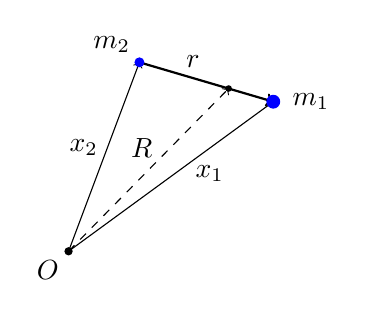
\begin{tikzpicture}[scale=1.0]
	\fill (0, 0) circle (1.5pt) node [below left] {$O$};
	\draw [->] (0, 0) -- (2.6, 1.9) node [pos = 0.6, below right = -2pt] {$\vv x_1$};
	\draw [->] (0, 0) -- (0.9, 2.4) node [pos = 0.55, left] {$\vv x_2$};
	\draw [->, dashed] (0, 0) -- (2.033, 2.067) node [pos = 0.55, above left = -2pt] {$\vv R$};
	\draw [->, thick] (0.9, 2.4) -- (2.6, 1.9) node [pos = 0.4, above] {$\vv r$};
	\fill [blue] (2.6, 1.9) circle (2.5pt);
	\node at (2.72, 1.9) [right] {$m_1$};
	\fill [blue] (0.9, 2.4) circle (1.8pt);
	\node at (0.8, 2.5) [above left = -3pt] {$m_2$};
	\fill (2.033, 2.067) circle (1.2pt);
\end{tikzpicture}
\end{center}

With no external forces, we know $\ddot{\vv R} = \vv 0$, so the centre of mass moves uniformly and can be taken as the origin of an inertial frame. Meanwhile,
$$
\ddot{\vv r} = \ddot{\vv x}_1 - \ddot{\vv x}_2 = \frac{\vv F_{12}}{m_1} - \frac{\vv F_{21}}{m_2} = \left(\frac{1}{m_1} + \frac{1}{m_2}\right)\vv F_{12},
$$
which we can rewrite as
$$
\mu \ddot{\vv r} = \vv F_{12}(\vv r), \quad \text{where } \mu = \frac{m_1 m_2}{m_1 + m_2}
$$
is called the \vocab{reduced mass}. This is exactly the equation for a \emph{single} particle of mass $\mu$ at position $\vv r$ moving about a fixed centre of force -- which is the problem we solved in the orbits section! The two-body problem thus reduces entirely to the one-body Kepler problem, and one can check that the angular momentum and kinetic energy also split accordingly:
$$
\vv L = M \vv R \times \dot{\vv R} + \mu \vv r \times \dot{\vv r}, \quad T = \frac{1}{2}M|\dot{\vv R}|^2 + \frac{1}{2}\mu |\dot{\vv r}|^2.
$$

\begin{example}[Binary Orbits]
	For two bodies under mutual gravity, $\vv F_{12} = -Gm_1m_2 \hh r/|\vv r|^2$, so
	$$
	\mu \ddot{\vv r} = -\frac{Gm_1m_2}{|\vv r|^2}\hh r \implies \ddot{\vv r} = -\frac{GM}{|\vv r|^2}\hh r.
	$$
	So the \emph{separation} traces out a conic exactly as before, but with the total mass $M$ appearing in the force law. In the centre of mass frame, each body individually moves in an ellipse about the (fixed) centre of mass, with
	$$
	\vv x_1 = \frac{m_2}{M}\vv r, \quad \vv x_2 = -\frac{m_1}{M}\vv r,
	$$
	so the two ellipses are similar, scaled by the mass ratio, with the bodies always on opposite sides of the centre of mass. When $m_1 \ll m_2$ (a planet and the Sun), $\mu \approx m_1$ and the centre of mass sits essentially at the heavier body -- recovering our fixed-Sun approximation, with a small correction: the Sun itself executes a miniature ellipse. It is exactly this tiny stellar `wobble' that provided some of the first detections of planets around other stars.
\end{example}

\subsection{Collisions}

A \emph{collision} is an interaction between two bodies which is brief and localised: before and after, the bodies move freely. Whatever complicated internal forces act during the collision, they are internal, so the \emph{total momentum is always conserved}:
$$
m_1 \vv u_1 + m_2 \vv u_2 = m_1 \vv v_1 + m_2 \vv v_2,
$$
where $\vv u_i$ are velocities before and $\vv v_i$ after. Kinetic energy is a different matter -- it may be transferred into heat, sound or deformation. We distinguish:
\begin{itemize}
	\item \emph{Elastic collisions}, in which the total kinetic energy is also conserved;
	\item \emph{Inelastic collisions}, in which some kinetic energy is lost (a \emph{totally} inelastic collision being one in which the bodies coalesce).
\end{itemize}

\begin{example}[Elastic Collision in One Dimension]
	Let a particle of mass $m_1$ and velocity $u$ strike a stationary particle of mass $m_2$, elastically, in one dimension.
	\begin{center}
	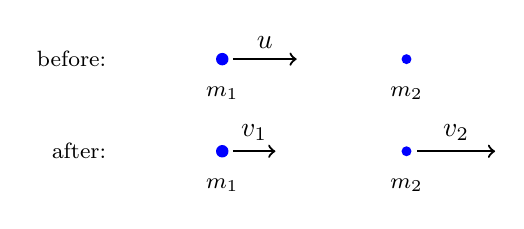
\begin{tikzpicture}[scale=0.9]
		\node at (-1.5, 1.3) [left] {\footnotesize before:};
		\fill [blue] (0, 1.3) circle (2.5pt);
		\node at (0, 1.05) [below] {\footnotesize $m_1$};
		\draw [->, thick] (0.15, 1.3) -- (1.05, 1.3) node [pos = 0.5, above] {$u$};
		\fill [blue] (2.6, 1.3) circle (2pt);
		\node at (2.6, 1.05) [below] {\footnotesize $m_2$};
		\node at (-1.5, 0) [left] {\footnotesize after:};
		\fill [blue] (0, 0) circle (2.5pt);
		\node at (0, -0.25) [below] {\footnotesize $m_1$};
		\draw [->, thick] (0.15, 0) -- (0.75, 0) node [pos = 0.5, above] {$v_1$};
		\fill [blue] (2.6, 0) circle (2pt);
		\node at (2.6, -0.25) [below] {\footnotesize $m_2$};
		\draw [->, thick] (2.75, 0) -- (3.85, 0) node [pos = 0.5, above] {$v_2$};
	\end{tikzpicture}
	\end{center}
	Conservation of momentum and energy give
	$$
	m_1 u = m_1 v_1 + m_2 v_2, \quad \frac{1}{2}m_1 u^2 = \frac{1}{2}m_1 v_1^2 + \frac{1}{2}m_2 v_2^2.
	$$
	Rearranging the first as $m_1(u - v_1) = m_2 v_2$ and the second as $m_1 (u - v_1)(u + v_1) = m_2 v_2^2$, then dividing (assuming a genuine collision, $v_2 \neq 0$), we get $u + v_1 = v_2$, and hence
	$$
	v_1 = \frac{m_1 - m_2}{m_1 + m_2}u, \quad v_2 = \frac{2m_1}{m_1 + m_2} u.
	$$
	The limiting cases are instructive. If $m_1 = m_2$, then $v_1 = 0$ and $v_2 = u$: the particles simply exchange velocities, as anyone who has played snooker knows. If $m_2 \gg m_1$ (a ball bouncing off a wall), $v_1 \approx -u$: the light particle bounces straight back. If $m_1 \gg m_2$, the heavy particle barrels on essentially unaffected, and the light one is flung ahead at $v_2 \approx 2u$.
\end{example}

\begin{example}[Totally Inelastic Collision]
	If instead the two particles coalesce, momentum conservation alone determines the outcome:
	$$
	v = \frac{m_1 u}{m_1 + m_2}.
	$$
	The kinetic energy lost is
	$$
	\Delta T = \frac{1}{2}m_1 u^2 - \frac{1}{2}(m_1 + m_2)v^2 = \frac{1}{2}\mu u^2,
	$$
	where $\mu$ is the reduced mass -- precisely the kinetic energy of the \emph{relative} motion. This makes sense: the centre of mass motion cannot be destroyed (momentum conservation), so the most energy a collision can possibly dissipate is the internal part, and a totally inelastic collision dissipates exactly that.
\end{example}

In higher dimensions, the same conservation laws apply, but they no longer determine the outcome uniquely -- the scattering angle remains free. A classic result: for an elastic collision between \emph{equal} masses, one initially at rest, conservation of momentum gives $\vv u_1 = \vv v_1 + \vv v_2$, and conservation of energy gives $|\vv u_1|^2 = |\vv v_1|^2 + |\vv v_2|^2$. Squaring the first equation and comparing, $\vv v_1 \cdot \vv v_2 = 0$: the particles move off \emph{at right angles} (unless one of them is at rest). We will revisit this in special relativity, where the right angle closes up.

\begin{remark}
	Real collisions sit between the elastic and totally inelastic extremes. A common phenomenological model (`Newton's experimental law') assigns a collision a \emph{coefficient of restitution} $e \in [0, 1]$: the relative velocity of separation is $e$ times the relative velocity of approach. Then $e = 1$ is the elastic case, $e = 0$ the totally inelastic one, and one can check that the kinetic energy lost is $\frac{1}{2}\mu (1 - e^2) |\vv u_1 - \vv u_2|^2$, interpolating between our two examples.
\end{remark}

\subsection{Variable Mass Problems \& The Rocket Equation}

Newton's second law reads $\dot{\vv p} = \vv F$ with $\vv p = m \vv v$ -- and nothing in it requires $m$ to be constant. Systems that gain or lose mass are everywhere: rockets burning fuel, raindrops accreting from a cloud, snowballs rolling downhill. The subtlety is that the mass that leaves (or joins) carries momentum with it, so we must be careful to apply the second law to a fixed collection of matter.

Consider the classic case: a rocket of mass $m(t)$ moving in a straight line with velocity $v(t)$, propelling itself by ejecting exhaust backwards with speed $u$ \emph{relative to the rocket}.

\begin{center}
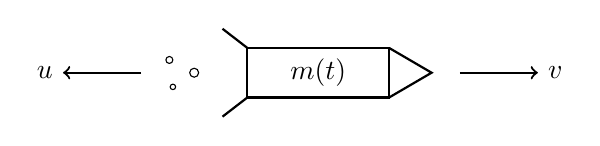
\begin{tikzpicture}[scale=0.9]
	\draw [thick] (0, -0.35) -- (2, -0.35) -- (2, 0.35) -- (0, 0.35) -- cycle;
	\draw [thick] (2, -0.35) -- (2.6, 0) -- (2, 0.35);
	\draw [thick] (0, 0.35) -- (-0.35, 0.62);
	\draw [thick] (0, -0.35) -- (-0.35, -0.62);
	\node at (1, 0) {$m(t)$};
	\draw [->, thick] (3.0, 0) -- (4.1, 0) node [right] {$v$};
	\draw (-0.75, 0) circle (1.8pt);
	\draw (-1.1, 0.18) circle (1.4pt);
	\draw (-1.05, -0.2) circle (1.1pt);
	\draw [->, thick] (-1.5, 0) -- (-2.6, 0) node [left] {$u$};
\end{tikzpicture}
\end{center}

Consider the total system of rocket plus exhaust between times $t$ and $t + \delta t$. At time $t$, the momentum is $m(t)v(t)$. At time $t + \delta t$, the rocket has mass $m(t + \delta t)$ and velocity $v(t + \delta t)$, and the mass $m(t) - m(t + \delta t)$ of ejected exhaust travels with velocity $v(t) - u + O(\delta t)$. So the change in total momentum is
\begin{align*}
	\delta p &= m(t + \delta t)v(t + \delta t) + \left[m(t) - m(t+\delta t)\right]\left[v(t) - u\right] - m(t)v(t) + O(\delta t^2)\\
	&= (m + \dot{m}\delta t)(v + \dot{v}\delta t) - \dot{m}\delta t (v - u) - mv + O(\delta t^2)\\
	&= (m \dot{v} + \dot{m} u)\, \delta t + O(\delta t^2).
\end{align*}
Newton's second law applied to the whole system (whose total mass \emph{is} constant) says $\delta p / \delta t \to F$, the external force on the rocket. We obtain:

\begin{proposition}[The Rocket Equation]
	$$
	m \frac{\dd v}{\dd t} + u \frac{\dd m}{\dd t} = F.
	$$
\end{proposition}

Note $\dot{m} < 0$ for a rocket, so the second term acts as a forward thrust of magnitude $u|\dot m|$.

\begin{example}[Rocket in Free Space]
	In deep space, $F = 0$, and taking the exhaust speed $u$ constant,
	$$
	m \frac{\dd v}{\dd t} = -u \frac{\dd m}{\dd t} \implies \frac{\dd v}{\dd m} = -\frac{u}{m} \implies v = v_0 + u \log\left(\frac{m_0}{m}\right),
	$$
	the \emph{Tsiolkovsky rocket equation}. Two features deserve comment. First, the final velocity depends only on the exhaust speed and the fraction of mass burnt -- not on \emph{how fast} the fuel is burnt. Second, the dependence on the mass ratio is only logarithmic, which is the tyranny of rocketry: to gain speed $u \log 10 \approx 2.3u$, ninety percent of your initial mass must be fuel. This is why real rockets are almost entirely fuel tank, and why they shed stages as they climb -- dropping an empty tank of mass $m_{\text{tank}}$ improves every subsequent burn's mass ratio, and multi-stage rockets squeeze substantially more final velocity out of the same fuel.
\end{example}

\begin{example}[A Falling Raindrop]
	For a raindrop falling through a stationary cloud and accreting mass, the accreted mass is at rest, so relative to the drop it arrives with speed $u = v$ (opposing the motion). With gravity as the external force, the rocket equation gives
	$$
	m \frac{\dd v}{\dd t} + v\frac{\dd m}{\dd t} = \frac{\dd}{\dd t}(m v) = mg,
	$$
	that is, the momentum $mv$ grows at rate $mg$. To go further we need a model for the accretion rate; for instance, if $\dot m = k m v$ (sweeping up mass in proportion to the volume swept out), one can show the drop approaches a constant terminal \emph{acceleration} of $g/7$ -- a fun exercise.
\end{example}



\section{Rigid Bodies} \label{sec:rigid}

In many cases, we want to study a system of particles such that the particles are constrained such that their relative positions are fixed. Such systems correspond to solid objects that cannot deform, break or bend.
Such systems are called \emph{rigid bodies}. Everything we established for general systems of particles -- the motion of the centre of mass, $\dot{\vv P} = \vv F^{\text{ext}}$ and $\dot{\vv L} = \vv \tau^{\text{ext}}$, the decompositions of energy and angular momentum -- applies verbatim; what the rigidity constraint buys us is that the internal motion is always a \emph{rotation}, so the whole configuration is captured by just a position and an orientation.

\subsection{Angular Velocity}

Suppose a rigid body $\BB$ is rotating about a fixed axis with angular speed $\omega$. If $\hh n$ is the unit vector parallel to the rotation axis, we define the \emph{vector angular velocity} of $\BB$ to be
$$
\vv \omega = \omega \hh n,
$$
where we choose the sign such that a positive $\omega$ corresponds to a right-handed rotation about the axis in the direction $\hh n$.

If $P$ is a particle in the rigid body $\BB$, then its velocity due to the rotation of the body is given by
$$
\vv v = \vv \omega \times (\vv r - \vv b),
$$
where $\vv b$ is the position vector corresponding to any fixed point $B$ on the rotation axis.

\subsection{Moment of Inertia}

Now suppose we have a rigid body made up of $N$ particles, rotating with angular velocity $\vv \omega$. Then we could write down the kinetic energy for the rigid body as
$$
T = \frac{1}{2} \sum_{i} m_i  \dot{\vv x_i} \cdot \dot{\vv x_i} = \frac{1}{2}I \omega^2,
$$
where
$$
I = \sum_{i = 1}^N m_i d_i^2
$$
is the \vocab{moment of inertia}, and $d_i$ is the perpendicular distance from particle $i$ to the axis of rotation.

The intuition behind moments of inertia is that they are to rotations what mass is to translations: the larger $I$ is, the more energy you need to supply to the body to make it spin.

\subsection{Angular Momentum and Moments of Inertia}

Recall that the angular momentum of a body is
$$
\vv L = \sum_i m_i \vv x_i \times  \dot{\vv x_i}.
$$
Suppose that the body is rotating with angular velocity $\omega \hh n$ about an axis through the origin. Then the component of angular momentum in the $\hh n$ direction is given by
\begin{align*}
	\vv L \cdot \hh n &= \sum_i m_i \vv x_i \times (\vv \omega \times \vv x_i) \cdot \hh n \\
	&= \omega \sum_i m_i (\vv x_i \times \hh n) \cdot (\vv x_i \times \hh n) \\
	&= I \omega,
\end{align*}
since $|\vv x_i \times \hh n| = d_i$, the perpendicular distance of particle $i$ from the axis. (The components of $\vv L$ perpendicular to $\hh n$ need not vanish, and in general $\vv L$ is \emph{not} parallel to $\vv \omega$ -- but we will not need this complication in this course.)
If there's a torque $\tau$ acting on the rigid body in the same direction as the angular velocity, so $\vv \tau = \tau \hh n$, then $I \dot{\omega} = \tau$.

\subsection{Calculating Moments of Inertia}

If we consider the rigid body as a continuous object with density distribution $\rho (\vv x)$, then the sums of the previous section become integrals, and the moment of inertia is given by
$$
I = \int \rho (\vv x)\, x_{\perp}^2 \dd V,
$$
where $x_\perp$ is the perpendicular distance from $\vv x$ to the axis of rotation. Let's compute a few of the standard examples properly.

\begin{example}[Thin Rod]
	Take a uniform thin rod of mass $M$ and length $2a$, rotating about an axis through its centre, perpendicular to the rod.
	\begin{center}
	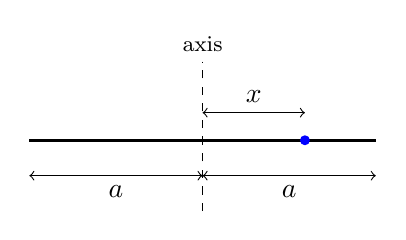
\begin{tikzpicture}[scale=1.0]
		\draw [dashed] (0, -0.9) -- (0, 1.0);
		\node at (0, 1.0) [above] {\footnotesize axis};
		\draw [very thick] (-2.2, 0) -- (2.2, 0);
		\fill [blue] (1.3, 0) circle (1.8pt);
		\draw [<->] (0, 0.35) -- (1.3, 0.35) node [pos = 0.5, above] {$x$};
		\draw [<->] (-2.2, -0.45) -- (0, -0.45) node [pos = 0.5, below] {$a$};
		\draw [<->] (0, -0.45) -- (2.2, -0.45) node [pos = 0.5, below] {$a$};
	\end{tikzpicture}
	\end{center}
	The mass per unit length is $\rho = M/2a$, and a point at position $x \in [-a, a]$ along the rod is at distance $|x|$ from the axis. So
	$$
	I = \int_{-a}^{a} \frac{M}{2a} x^2 \dd x = \frac{M}{2a}\cdot \frac{2a^3}{3} = \frac{1}{3}Ma^2.
	$$
\end{example}

\begin{example}[Circular Hoop and Disc]
	For a hoop of mass $M$ and radius $a$, about the axis through its centre perpendicular to its plane, every point is at distance exactly $a$ from the axis, so immediately $I = Ma^2$.

	For a uniform disc of mass $M$ and radius $a$ about the same axis, the surface density is $\rho = M/\pi a^2$, and working in plane polar coordinates with area element $r \dd r \dd\theta$,
	$$
	I = \int_0^{2\pi}\!\!\int_0^a \frac{M}{\pi a^2}\, r^2 \cdot r \dd r \dd \theta = \frac{M}{\pi a^2} \cdot 2\pi \cdot \frac{a^4}{4} = \frac{1}{2}Ma^2.
	$$
	\begin{center}
	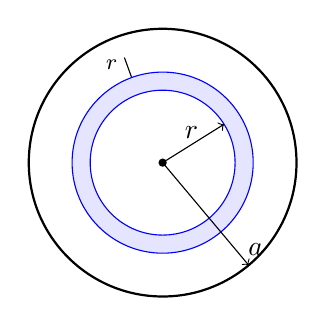
\begin{tikzpicture}[scale=1.0]
		\filldraw [fill=blue!10, draw=blue, even odd rule] (0, 0) circle (1.15) (0, 0) circle (0.92);
		\draw [thick] (0, 0) circle (1.7);
		\fill (0, 0) circle (1.5pt);
		\draw [->] (0, 0) -- (32:0.92) node [pos = 0.6, above left = -3pt] {$r$};
		\draw [->] (0, 0) -- (-50:1.7) node [pos = 0.85, right = 1pt] {$a$};
		\draw (110:1.16) -- (110:1.42);
		\node at (110:1.32) [left] {\footnotesize $\dd r$};
	\end{tikzpicture}
	\end{center}
	Here we have summed over rings of radius $r$ and thickness $\dd r$ (shaded), each of which contributes mass at a common distance $r$ from the axis.
\end{example}

\begin{example}[Solid Sphere]
	For a uniform solid sphere of mass $M$ and radius $a$ about an axis through its centre, take the axis to be the $z$-axis and use the density $\rho = 3M/4\pi a^3$. Slicing the sphere into discs of thickness $\dd z$ at height $z$, each of radius $\sqrt{a^2 - z^2}$, and using the disc result,
	$$
	I = \int_{-a}^{a} \frac{1}{2}\left(\rho \pi (a^2 - z^2)\right)(a^2 - z^2)\dd z = \frac{\rho \pi}{2}\int_{-a}^a (a^2 - z^2)^2 \dd z = \frac{\rho\pi}{2}\cdot\frac{16a^5}{15} = \frac{2}{5}Ma^2.
	$$
\end{example}

Collecting these (all worth remembering):
\begin{enumerate}
	\item \emph{Thin Rod}. With mass $M$ and length $2a$, about an axis perpendicular to the rod through its centre: $I = \frac{1}{3}M a^2$.
	\item \emph{Circular Hoop}. With mass $M$ and radius $a$, about an axis perpendicular to the plane of the hoop through its centre: $I = Ma^2$.
	\item \emph{Circular Disc}. With mass $M$ and radius $a$, about an axis perpendicular to the plane of the disc through its centre: $I = \frac{1}{2}Ma^2$.
	\item \emph{Solid Sphere}. With mass $M$ and radius $a$, about an axis through its centre: $I = \frac{2}{5}Ma^2$.
\end{enumerate}

Two general theorems let us transport these results to other axes without redoing any integrals.

\begin{theorem}[Parallel Axis Theorem]
	If a rigid body of mass $M$ has moment of inertia $I_G$ about an axis through its centre of mass, then its moment of inertia about a parallel axis a distance $d$ away is
	$$
	I = I_G + Md^2.
	$$
\end{theorem}
\begin{proof}
	Set up coordinates with origin at the centre of mass and the first axis along $\vv e_z$, and let the parallel axis pass through the point $d \vv e_x$. Writing $\vv x_i = (x_i, y_i, z_i)$ for the particles of the body, the perpendicular distance from particle $i$ to the new axis satisfies $d_i'^2 = (x_i - d)^2 + y_i^2$. So
	$$
	I = \sum_i m_i \left((x_i - d)^2 + y_i^2\right) = \sum_i m_i (x_i^2 + y_i^2) - 2d \sum_i m_i x_i + d^2 \sum_i m_i = I_G + Md^2,
	$$
	where the middle sum vanishes because the centre of mass is at the origin.
\end{proof}

Note in particular that $I \geq I_G$: of all axes in a given direction, the one through the centre of mass gives the smallest moment of inertia.

\begin{theorem}[Perpendicular Axis Theorem]
	For a two dimensional body (a \emph{lamina}) lying in the $(x,y)$ plane, the moments of inertia about the coordinate axes satisfy
	$$
	I_z = I_x + I_y.
	$$
\end{theorem}
\begin{proof}
	Since $z_i = 0$ for every particle, we have $I_x = \sum m_i y_i^2$ and $I_y = \sum_i m_i x_i^2$, while $I_z = \sum_i m_i (x_i^2 + y_i^2) = I_x + I_y$.
\end{proof}

\begin{example}
	For the uniform disc, by symmetry $I_x = I_y$, and $I_z = \frac{1}{2}Ma^2$ from before. So the moment of inertia of a disc about one of its \emph{diameters} is $I_x = \frac{1}{4}Ma^2$ -- no integration required. Similarly, using the parallel axis theorem, a rod of length $2a$ spun about one of its \emph{ends} has $I = \frac{1}{3}Ma^2 + Ma^2 = \frac{4}{3}Ma^2$.
\end{example}

\begin{example}[Rectangular Lamina]
	For a uniform rectangular plate of mass $M$ with sides $2a$ and $2b$, the moment of inertia about the in-plane axis through the centre parallel to the side of length $2b$ only `sees' the $x$-extent of the mass, so it equals that of a rod: $I_y = \frac{1}{3}Ma^2$, and likewise $I_x = \frac{1}{3}Mb^2$. The perpendicular axis theorem then gives, for the axis through the centre perpendicular to the plate,
	$$
	I_z = I_x + I_y = \frac{1}{3}M(a^2 + b^2),
	$$
	with all three answers obtained from a single one dimensional integral.
\end{example}

\subsection{Motion of Rigid Bodies}

The general motion of a rigid body is a translation of its centre of mass along some trajectory $\vv R(t)$, together with a rotation about an axis through the centre of mass. Writing $\vv x_i = \vv R + \vv y_i$ as in Section~\ref{sec:systems}, the rigidity constraint means the relative positions $\vv y_i$ evolve by pure rotation, so
$$
\dot{\vv x}_i = \dot{\vv R} + \vv \omega \times \vv y_i
$$
for some angular velocity $\vv \omega(t)$. Our kinetic energy decomposition then becomes
$$
T = \frac{1}{2}M |\dot{\vv R}|^2 + \frac{1}{2}\sum_i m_i |\vv \omega \times \vv y_i|^2 = \underbrace{\frac{1}{2}M|\dot{\vv R}|^2}_{\text{translational}} + \underbrace{\frac{1}{2}I_G\, \omega^2}_{\text{rotational}},
$$
where $I_G$ is the moment of inertia about the axis through the centre of mass in the direction of $\vv \omega$. The motion is governed by our two equations for systems of particles,
$$
\dot{\vv P} = \vv F^{\text{ext}}, \quad \dot{\vv L} = \vv \tau^{\text{ext}},
$$
where the angular momentum and torque may be taken about any fixed point of an inertial frame, \emph{or} about the centre of mass -- the latter works even when the centre of mass is accelerating, since the fictitious forces this introduces have zero net torque about the centre of mass.\footnote{In the accelerating centre of mass frame, each particle feels a fictitious force $-m_i \ddot{\vv R}$, and the total torque of these about the centre of mass is $-\left(\sum_i m_i \vv y_i\right) \times \ddot{\vv R} = \vv 0$.}

In a \emph{uniform} gravitational field, the external force and torque take a particularly nice form:
$$
\vv F = \sum_i m_i \vv g = M \vv g, \quad \vv \tau = \sum_i \vv x_i \times m_i \vv g = M \vv R \times \vv g.
$$
Both are exactly what would act on a single particle of mass $M$ at the centre of mass. In particular, the gravitational torque \emph{about} the centre of mass vanishes.

\begin{example}[A Thrown Stick]
	Throw a uniform stick spinning through the air (ignoring air resistance). The centre of mass traces a parabola, exactly as a point particle would. Meanwhile, since gravity exerts no torque about the centre of mass, $\dot{\vv L}^{\text{CoM}} = \vv 0$, and the stick rotates with constant angular velocity about its centre as it flies.
\end{example}

\subsection{The Compound Pendulum}

Our equation for rotation about a fixed axis is already enough to handle a classic example -- a pendulum made from an arbitrary rigid body.

\begin{example}[The Compound Pendulum]
	A rigid body is free to swing under gravity in a vertical plane about a fixed horizontal axis through a point $P$, which is a distance $d$ from the centre of mass $G$. Let $\theta$ be the angle of $PG$ from the downward vertical, and let $I$ be the moment of inertia of the body about the axis through $P$ (computable via the parallel axis theorem: $I = I_G + Md^2$).
	\begin{center}
	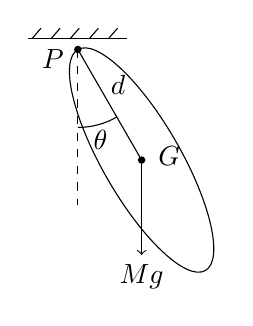
\begin{tikzpicture}[scale=0.9]
		\draw (-0.7, 0.15) -- (0.7, 0.15);
		\foreach \x in {-0.65, -0.38, -0.11, 0.16, 0.43} \draw (\x, 0.15) -- (\x + 0.13, 0.3);
		\fill (0, 0) circle (1.5pt);
		\node at (-0.06, -0.14) [left] {$P$};
		\draw [rotate around = {30:(0.9, -1.56)}] (0.9, -1.56) ellipse (0.55 and 1.8);
		\fill (0.9, -1.56) circle (1.5pt);
		\node at (1.0, -1.5) [right] {$G$};
		\draw (0, 0) -- (0.9, -1.56) node [pos = 0.45, above right = -2pt] {$d$};
		\draw [dashed] (0, 0) -- (0, -2.2);
		\draw (0, -1.1) arc (270:300:1.1);
		\node at (0.32, -1.28) {$\theta$};
		\draw [->] (0.9, -1.56) -- (0.9, -2.9) node [below] {$M \vv g$};
	\end{tikzpicture}
	\end{center}
	The body rotates about the fixed point $P$, so $L = I \dot\theta$, and the torque about $P$ is due to gravity acting at the centre of mass:
	$$
	I \ddot{\theta} = -Mgd \sin \theta.
	$$
	This is exactly the simple pendulum equation, so all our pendulum analysis applies: small oscillations have angular frequency
	$$
	\omega = \sqrt{\frac{Mgd}{I}},
	$$
	i.e.\ the body behaves as a simple pendulum of \emph{effective length} $\ell_{\text{eff}} = I/Md$.

	For instance, for a uniform rod of length $\ell$ pivoted at one end, we have $d = \ell/2$ and (from our earlier example, with $2a = \ell$) $I = \frac{1}{3}M\ell^2$, so
	$$
	\ddot{\theta} = -\frac{3g}{2\ell}\sin\theta,
	$$
	and the rod swings like a simple pendulum of length $2\ell/3$. The same equation drops out of energy conservation: differentiating $E = \frac{1}{2}I \dot\theta^2 - Mgd\cos\theta$ with respect to time and cancelling $\dot\theta$ recovers the equation of motion.
\end{example}

\begin{example}[The Centre of Percussion]
	Here is a question every cricketer cares about: where should the ball strike the bat so that your hands feel no jarring? Model the bat as a uniform rod of mass $M$ and length $\ell$, held (pivoted) at one end, and suppose the ball delivers a sharp horizontal impulse $J$ at a distance $b$ from the pivot. During the blow, the pivot exerts some impulsive reaction $R$ on the rod.

	Take angular impulse about the pivot (about which $I = \frac{1}{3}M\ell^2$): the reaction has no moment there, so
	$$
	I\, \Delta\omega = J b \implies \Delta \omega = \frac{Jb}{I}.
	$$
	Meanwhile the linear impulse determines the change in velocity of the centre of mass, which sits at $d = \ell/2$ from the pivot and moves with velocity $d\,\Delta\omega$ after the blow:
	$$
	J + R = M d\, \Delta\omega = \frac{MdJb}{I} \implies R = J\left(\frac{Mdb}{I} - 1\right).
	$$
	The reaction at the hands vanishes exactly when
	$$
	b = \frac{I}{Md} = \frac{\frac{1}{3}M\ell^2}{M \ell/2} = \frac{2\ell}{3}.
	$$
	This point is called the \vocab{centre of percussion} -- strike there and the bat pivots cleanly about your hands with no sting; strike elsewhere and $R \neq 0$, which your palms report immediately. Note it is the same point $2\ell/3$ that appeared as the `effective length' of the swinging rod, which is no coincidence: both are the point where the rod behaves like an equivalent simple pendulum.
\end{example}

\subsection{Rolling Without Slipping}

Consider a circular object -- a cylinder, hoop or sphere -- of radius $a$, moving along a surface, with its centre moving at speed $v$ and the body rotating at angular speed $\omega$ about its centre. The velocity of the material point of the body instantaneously in contact with the surface is
$$
v_{\text{slip}} = v - a\omega.
$$
There are two qualitatively different regimes:
\begin{itemize}
	\item \emph{Sliding}: $v_{\text{slip}} \neq 0$. The contact point scrapes along the surface, kinetic friction $\mu N$ acts to oppose the slipping, and mechanical energy is dissipated.
	\item \emph{Rolling}: $v_{\text{slip}} = 0$, i.e.\ $v = a\omega$. This is the \vocab{rolling without slipping} condition. The contact point is instantaneously stationary -- so although friction may act (and is often what \emph{enforces} rolling), it acts at a point moving with zero velocity, and hence \emph{does no work}. Energy is conserved for rolling bodies.
\end{itemize}
A rolling body can equivalently be viewed as rotating with angular speed $\omega$ about the (instantaneously stationary) contact point.

\begin{center}
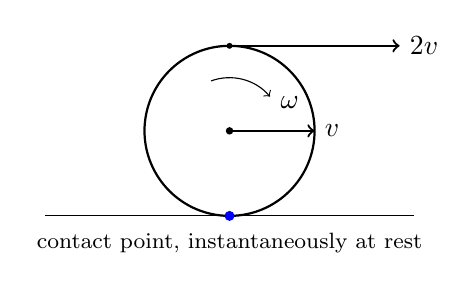
\begin{tikzpicture}[scale=0.9]
	\draw (-2.6, 0) -- (2.6, 0);
	\draw [thick] (0, 1.2) circle (1.2);
	\fill (0, 1.2) circle (1.5pt);
	\draw [->, thick] (0, 1.2) -- (1.2, 1.2) node [right] {$v$};
	\fill (0, 2.4) circle (1.2pt);
	\draw [->, thick] (0, 2.4) -- (2.4, 2.4) node [right] {$2v$};
	\draw [->] (-0.26, 1.905) arc (110:40:0.75);
	\node at (0.85, 1.6) {$\omega$};
	\fill [blue] (0, 0) circle (2pt);
	\node at (0, -0.1) [below] {\footnotesize contact point, instantaneously at rest};
\end{tikzpicture}
\end{center}

\begin{example}[Rolling Down a Slope]
	A uniform cylinder or sphere of mass $M$, radius $a$ and moment of inertia $I$ (about its axis through the centre of mass) rolls without slipping down a plane inclined at angle $\alpha$. Let $x$ be the distance travelled down the slope, so the rolling condition gives $\omega = \dot{x}/a$. The energy
	$$
	E = \frac{1}{2}M\dot{x}^2 + \frac{1}{2}I \omega^2 - Mgx \sin\alpha = \frac{1}{2}\left(M + \frac{I}{a^2}\right)\dot{x}^2 - Mg x \sin \alpha
	$$
	is conserved (friction does no work while rolling), so differentiating and cancelling $\dot{x}$,
	$$
	\ddot{x} = \frac{g \sin\alpha}{1 + I/Ma^2}.
	$$
	The body accelerates more slowly than the sliding value $g \sin\alpha$, because some of the released potential energy must be spent spinning it up. The acceleration depends only on the \emph{shape} through the ratio $I/Ma^2$: a solid sphere ($I = \frac{2}{5}Ma^2$) has $\ddot x = \frac{5}{7}g\sin\alpha$, a solid cylinder ($\frac{1}{2}Ma^2$) has $\frac{2}{3}g\sin\alpha$, and a hoop ($Ma^2$) has $\frac{1}{2}g \sin\alpha$. So in a race down a hill, the sphere beats the cylinder, which beats the hoop, with the masses and radii entirely irrelevant. The same result follows from the force/torque equations $M\dot v = Mg\sin\alpha - F$ and $I \dot\omega = aF$, where $F$ is the friction force enforcing the rolling.
\end{example}

\begin{example}[The Struck Snooker Ball]
	A snooker ball (a uniform sphere, $I = \frac{2}{5}Ma^2$) is struck centrally, so it initially translates with speed $v_0$ but does not spin: $v = v_0$, $\omega = 0$, and so $v_{\text{slip}} = v_0 > 0$. The ball is sliding, so kinetic friction $F = \mu_k M g$ acts backwards at the contact point, and
	$$
	M \dot{v} = -\mu_k Mg, \quad I \dot{\omega} = a \mu_k M g.
	$$
	So the ball slows down while spinning up:
	$$
	v(t) = v_0 - \mu_k g t, \quad a\omega(t) = \frac{5}{2}\mu_k g t,
	$$
	and the slip velocity $v_{\text{slip}} = v_0 - \frac{7}{2}\mu_k g t$ decreases to zero at time $t_{\text{roll}} = \frac{2 v_0}{7 \mu_k g}$. At that moment $v = a\omega = \frac{5}{7}v_0$, rolling begins, friction ceases to act (no applied force, no tendency to slip), and the ball rolls on at constant speed $\frac{5}{7}v_0$. The kinetic energy at this point is
	$$
	\frac{1}{2}\left(M + \frac{I}{a^2}\right)v^2 = \frac{7}{10}M \cdot \frac{25}{49}v_0^2 = \frac{5}{14}Mv_0^2 < \frac{1}{2}Mv_0^2,
	$$
	the difference having been dissipated by friction during the sliding phase.
\end{example}

\begin{example}[When Does Rolling Fail?]
	Return to the body on the inclined plane, and ask: how steep can the slope be before rolling becomes impossible? While rolling, the friction force required to sustain the motion is, from the equations $M \dot v = Mg\sin\alpha - F$ and $I \dot\omega = aF$ with $\dot v = a \dot \omega$,
	$$
	F = \frac{I/a^2}{M + I/a^2}\, Mg \sin\alpha.
	$$
	But static friction can supply at most $\mu N = \mu Mg \cos\alpha$. So rolling is sustainable only if
	$$
	\tan \alpha \leq \mu\left(1 + \frac{Ma^2}{I}\right).
	$$
	On steeper slopes the contact point must slip, and the body slides as it spins. Note the shape-dependence again: a hoop ($I = Ma^2$) demands the most friction and starts slipping first, while a solid sphere holds on to steeper slopes.
\end{example}
\section{Special Relativity} \label{sec:sr}

We now leave Newtonian mechanics behind. The trouble began with electromagnetism: Maxwell's equations predict that light travels at a definite speed $c \approx \SI{3e8}{\meter\per\second}$ -- but a speed relative to \emph{what}? Under Galilean transformations, velocities simply add, so different inertial observers should measure different speeds of light, and experiments (most famously that of Michelson and Morley) resolutely failed to detect any such difference. Einstein's 1905 resolution was radical: keep the principle of relativity, keep the constancy of the speed of light, and let our assumptions about space and time -- including Galilean transformations and absolute time itself -- fall where they may.

\subsection{Axioms of Special Relativity}

The whole of special relativity is built upon two deceptively simple postulates.

\begin{axiom}[Postulates of Special Relativity]
	\begin{enumerate}
		\item \emph{Principle of relativity}. The laws of physics are the same in all inertial reference frames.
		\item \emph{Constancy of the speed of light}. The speed of light in a vacuum is the same in all inertial reference frames.
	\end{enumerate}
\end{axiom}

The first postulate is just Galilean relativity as before. The second sounds innocuous but is flatly incompatible with the Galilean transformations: if a light ray passes you at speed $c$, and I chase after it at speed $c/2$, the second postulate insists that I \emph{also} measure the light receding at speed $c$, not $c/2$. Clearly velocity addition -- and with it, our notions of time and length -- must be rebuilt from scratch.

\begin{aside}{Aside: The Michelson--Morley Experiment}
	Nineteenth-century physics held that light waves, like all other waves, must propagate in \emph{some} medium -- the `luminiferous ether' -- and that Maxwell's $c$ was the speed of light relative to it. The Earth, orbiting the Sun at about $\SI{30}{\kilo\meter\per\second}$, ought then to be moving through the ether, and light should travel at measurably different speeds in different directions.

	In 1887, Michelson and Morley set out to detect this using an interferometer: a light beam is split, sent down two perpendicular arms, reflected back, and recombined, with any difference in travel times showing up as a shift in the interference fringes as the apparatus is rotated. The expected effect was well within their sensitivity. They found \emph{nothing} -- no fringe shift, in any season, in any orientation. It is one of the most famous null results in the history of science.

	Various rescues were attempted, most notably by FitzGerald and Lorentz, who observed that the null result could be explained if objects moving through the ether contracted by a factor $\sqrt{1 - v^2/c^2}$ in their direction of motion -- the right formula, proposed as a mysterious dynamical accident. Einstein's 1905 insight was that no ether and no accident are needed: if the speed of light is simply the same in every inertial frame, the contraction (and much else) follows from the geometry of space and time itself. That is the theory we now develop.

\end{aside}

\subsection{Lorentz Transformations}

In special relativity we think in terms of \vocab{events}: instantaneous, point-like occurrences. These are specified by four coordinates, one of time and three of position, like $(t, x, y, z)$.
These coordinates will be measured differently in different inertial frames, and to make our axioms hold we need to use a new set of transformation laws.

Let $\FF$ and $\FF'$ be inertial frames, with $\FF'$ moving at speed $v$ relative to $\FF$ in the $x$ direction, in a \emph{standard configuration}: axes aligned, origins coinciding at $t = t' = 0$. What could the transformation between them look like? We will sketch how the axioms pin it down. First, the transformation must map unaccelerated motion to unaccelerated motion (both frames are inertial), and this forces it to be \emph{linear} in $(t, x)$. Motion transverse to the boost cannot be affected (by symmetry of the setup) so $y' = y$ and $z' = z$, and the origin of $\FF'$ (i.e.\ $x' = 0$) must move along $x = vt$, so
$$
x' = \gamma (x - vt)
$$
for some factor $\gamma(v)$. By the principle of relativity, the inverse transformation must take the same form with $v \mapsto -v$ (and the same $\gamma$, which can depend only on $|v|$, again by symmetry):
$$
x = \gamma(x' + vt').
$$
Now impose the second postulate: a light ray through the origin has $x = ct$ in $\FF$, and must also have $x' = ct'$ in $\FF'$. Substituting both into the two equations above,
$$
ct' = \gamma t (c - v), \quad ct = \gamma t'(c + v),
$$
and multiplying these together gives $c^2 = \gamma^2 (c - v)(c + v)$, so
$$
\gamma = \frac{1}{\sqrt{1 - v^2/c^2}},
$$
the famous \vocab{Lorentz factor}. Eliminating $x'$ between the two boxed-style relations then yields the transformation of time. The result is the \vocab{Lorentz transformation}:
\begin{align*}
	ct' &= \gamma\left(ct - \frac{v}{c}x\right) \\
	x' &= \gamma \left(x - \frac{v}{c}\, ct\right) \\
	y' &= y \\
	z' &= z.
\end{align*}
A few observations to orient ourselves.
\begin{enumerate}[label=(\roman*)]
	\item \emph{Time transforms.} The first line is the revolution: $t'$ depends on $x$ as well as $t$. Different frames genuinely disagree about time, and the disagreement grows with separation in space. Absolute time is gone.
	\item \emph{The Newtonian limit.} When $v/c$ is very small, $\gamma \approx 1$ and the transformations reduce to $x' = x - vt$, $t' = t$: the Galilean boost. All of Newtonian mechanics survives as the low-speed approximation, which is why it took humanity so long to notice anything was wrong.
	\item \emph{The speed limit.} The factor $\gamma$ is real only for $|v| < c$, and $\gamma \to \infty$ as $|v| \to c$. The speed of light is built into the geometry as a limiting speed for frames (and, as we will see, for particles).
	\item \emph{Symmetry.} The map treats $ct$ and $x$ almost symmetrically, mixing them rather like a rotation mixes coordinates -- a hint we will make precise when we study rapidity.
\end{enumerate}

\subsection{Spacetime Diagrams}

Relativity problems reward drawing pictures. A \vocab{spacetime diagram} plots position $x$ horizontally against time \emph{scaled as} $ct$ vertically (so that both axes carry dimensions of length). A point on the diagram is an event; the history of a particle traces out a curve called its \vocab{world line}. A particle at rest has a vertical world line; a particle in uniform motion has a straight world line tilted from the vertical; and a light ray has a world line at exactly $45\dg$, since it satisfies $x = \pm ct$.

\begin{center}
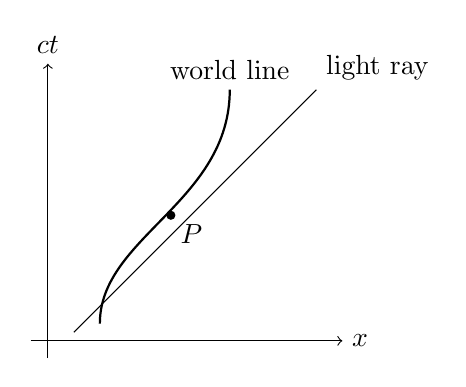
\begin{tikzpicture}[scale=1.1]
	\draw [->] (-0.2, 0) -- (3.4, 0) node [right] {$x$};
	\draw [->] (0, -0.2) -- (0, 3.2) node [above] {$ct$};
	\draw [thick] (0.6, 0.2) .. controls (0.6, 1.2) and (2.1, 1.6) .. (2.1, 2.9) node [above] {world line};
	\fill (1.42, 1.45) circle (1.5pt) node [below right] {$P$};
	\draw (0.3, 0.1) -- (3.1, 2.9) node [above right] {light ray};
\end{tikzpicture}
\end{center}

Now the crucial construction: how do the axes of a moving frame $\FF'$ appear on the diagram of $\FF$? The $ct'$ axis is the set of events with $x' = 0$, which is the line $x = vt$ -- a line through the origin with gradient $c/v > 1$, i.e.\ tilted from the vertical. The $x'$ axis is the set of events with $t' = 0$, which by the Lorentz transformation is the line $ct = \frac{v}{c}x$ -- tilted \emph{up} from the horizontal by the same angle. So the primed axes close in symmetrically, like a pair of scissors, about the $45\dg$ light ray:

\begin{center}
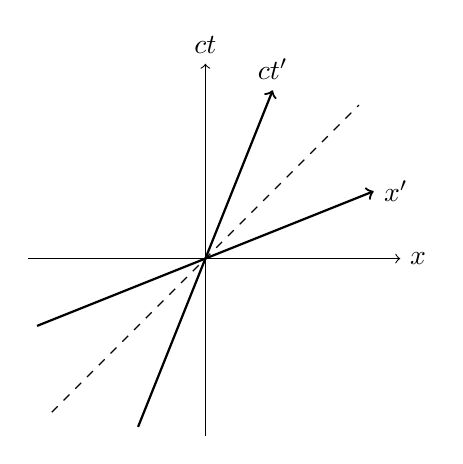
\begin{tikzpicture}[scale=0.75]
	\draw [->] (-3, 0) -- (3.3, 0) node [right] {$x$};
	\draw [->] (0, -3) -- (0, 3.3) node [above] {$ct$};
	\draw [->, thick] (-2.85, -1.14) -- (2.85, 1.14) node [right] {$x'$};
	\draw [->, thick] (-1.14, -2.85) -- (1.14, 2.85) node [above] {$ct'$};
	\draw [dashed] (-2.6, -2.6) -- (2.6, 2.6);
\end{tikzpicture}
\end{center}

The primed axes are \emph{not} orthogonal on the page -- but both frames agree on the world lines of light rays, which bisect the axes in each frame. Almost every counterintuitive result of the subject (the relativity of simultaneity, time dilation, length contraction) becomes nearly obvious once drawn on such a diagram, so we will use them liberally in what follows.

\subsection{Simultaneity}

We say two events $P_1$ and $P_2$ are \emph{simultaneous} in the frame $\FF$ if they have the same time coordinate $t$. On a spacetime diagram, the events simultaneous with a given event form a horizontal line -- a \emph{line of simultaneity} of $\FF$.

But the lines of simultaneity of $\FF'$ are the lines of constant $t'$, which by the Lorentz transformation are the lines
$$
ct - \frac{v}{c}x = \text{const},
$$
which are \emph{tilted} lines parallel to the $x'$ axis. Events with the same $t$ no longer correspond to events with equal $t'$, so what is simultaneous in one frame is not necessarily simultaneous in another.

\begin{center}
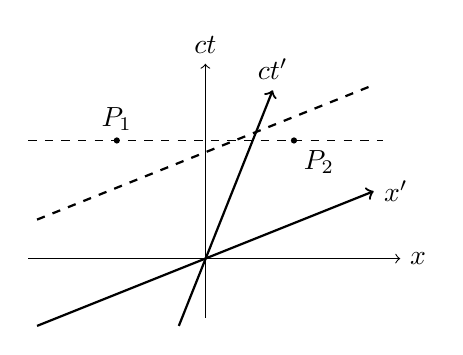
\begin{tikzpicture}[scale=0.75]
	\draw [->] (-3, 0) -- (3.3, 0) node [right] {$x$};
	\draw [->] (0, -1) -- (0, 3.3) node [above] {$ct$};
	\draw [dashed] (-3, 2) -- (3, 2);
	\fill (-1.5, 2) circle (1.5pt) node [above] {$P_1$};
	\fill (1.5, 2) circle (1.5pt) node [below right] {$P_2$};
	\draw [->, thick] (-2.85, -1.14) -- (2.85, 1.14) node [right] {$x'$};
	\draw [dashed, thick] (-2.85, 0.66) -- (2.85, 2.94);
	\draw [->, thick] (-0.45, -1.14) -- (1.14, 2.85) node [above] {$ct'$};
\end{tikzpicture}
\end{center}

In the diagram, $P_1$ and $P_2$ are simultaneous in $\FF$ (they lie on a horizontal dashed line), but the tilted line of simultaneity of $\FF'$ through $P_1$ passes \emph{above} $P_2$ -- so in $\FF'$, the event $P_2$ happens first. This is a genuine disagreement, not an artefact of light taking time to reach anyone's eyes: the coordinates already account for all such delays.

\subsection{Causality \& Light Cones}

If observers can disagree about the order of events, should we worry about effects preceding their causes? Consider an event $P$, which we may as well place at the origin. The light rays through $P$ divide spacetime into regions, and this division is \emph{frame independent}, since all observers agree on the speed of light:

\begin{center}
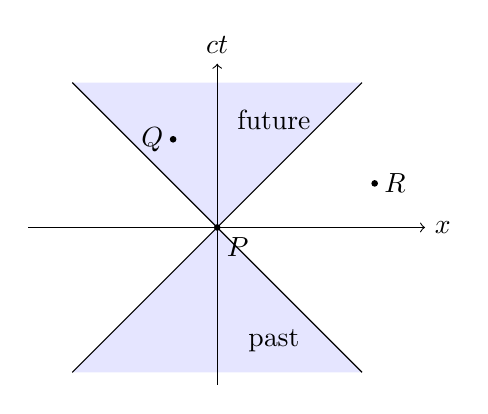
\begin{tikzpicture}[scale=0.8]
	\fill [blue!10] (-2.3, 2.5) -- (0, 0.2) -- (2.3, 2.5) -- cycle;
	\fill [blue!10] (-2.3, -2.1) -- (0, 0.2) -- (2.3, -2.1) -- cycle;
	\draw [->] (-3, 0.2) -- (3.3, 0.2) node [right] {$x$};
	\draw [->] (0, -2.3) -- (0, 2.8) node [above] {$ct$};
	\draw (-2.3, 2.5) -- (2.3, -2.1);
	\draw (2.3, 2.5) -- (-2.3, -2.1);
	\fill (0, 0.2) circle (1.5pt) node [below right] {$P$};
	\node at (0.9, 1.9) {future};
	\node at (0.9, -1.6) {past};
	\fill (-0.7, 1.6) circle (1.5pt) node [left] {$Q$};
	\fill (2.5, 0.9) circle (1.5pt) node [right] {$R$};
\end{tikzpicture}
\end{center}

The region $|x| \leq ct$ (shaded) is the \vocab{light cone} of $P$: the \emph{future light cone} consists of all events reachable from $P$ by influences travelling at up to the speed of light, and the \emph{past light cone} of all events that can influence $P$. For an event $Q$ inside the future light cone of $P$, one can check from the Lorentz transformation that \emph{every} inertial frame agrees that $Q$ occurs after $P$ -- so cause and effect are never inverted. For an event $R$ \emph{outside} the light cone, frames can disagree about the order of $P$ and $R$ (and there is even a frame in which they are simultaneous) -- but no signal travelling at speed at most $c$ can connect them, so neither can influence the other, and no causal paradox arises. Causality survives, provided nothing travels faster than light.

\subsection{Time Dilation}

Consider a clock sitting stationary at the origin of the frame $\FF'$, ticking at intervals of $T'$. The tick events in frame $\FF'$ occur at $(ct'_1, 0), (c(t'_1 + T'), 0), \dots$, all with $x' = 0$. Using the inverse Lorentz transformation $t = \gamma(t' + vx'/c^2)$ with $x' = 0$, the interval between ticks observed in $\FF$ is
$$
T = \gamma T' > T'.
$$
So the interval between ticks is longer in the frame in which the clock moves: \emph{moving clocks run slowly}. The effect is mutual -- a clock at rest in $\FF$ runs slowly as measured in $\FF'$ -- which sounds paradoxical, but the two statements compare different pairs of measurements, made along different lines of simultaneity, and no contradiction can be manufactured (as the twin `paradox' below illustrates).

\begin{example}[Muons in the Atmosphere]
	Muons are unstable particles with a lifetime of about $\SI{2.2}{\micro\second}$, created by cosmic rays striking the upper atmosphere, around $\SI{10}{\kilo\meter}$ up. Even travelling at essentially the speed of light, a muon should manage only about $c \times \SI{2.2}{\micro\second} \approx \SI{660}{\meter}$ before decaying -- yet muons are detected in abundance at sea level. The resolution is time dilation: for a muon with $\gamma \approx 20$, its internal clock ticks $20$ times slower as observed from the ground, giving it ample time to complete the journey. (From the muon's own point of view, its clock runs normally -- but, as we will see next, the atmosphere is length-contracted to a twentieth of its height.)

	Nor is time dilation exotic: the clocks on GPS satellites, orbiting at about $\SI{3.9}{\kilo\meter\per\second}$, run slow relative to the ground by around $7$ microseconds per day due to time dilation (partially offset by a general-relativistic effect of the weaker gravity up there). Uncorrected, the resulting positioning error would accumulate at kilometres per day -- your phone does relativity every time it finds you on a map.
\end{example}

\begin{example}[The Twin Paradox]
	Consider twins Alice and Bob. Bob stays at home (an inertial frame). Alice travels at constant speed $v$ to a distant star, a distance $d$ away in Bob's frame, then immediately turns around and returns at the same speed. In Bob's frame the journey takes $T = d/v$ each way, so Bob ages $2T$. Alice's clock, moving throughout, runs slow by a factor $\gamma$, so she ages only $2T/\gamma$: Alice returns \emph{genuinely younger} than her twin.

	The apparent paradox: from Alice's point of view, isn't it Bob who moves, so shouldn't Bob be younger? The asymmetry is that Bob remains inertial throughout while Alice does not -- she turns around, and the situation is not symmetric. The spacetime diagram makes it precise:
	\begin{center}
	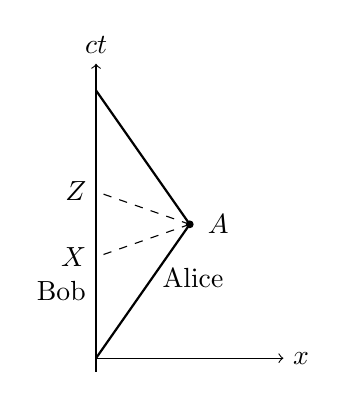
\begin{tikzpicture}[scale=0.85]
		\draw [->] (0, 0) -- (2.8, 0) node [right] {$x$};
		\draw [->] (0, -0.2) -- (0, 4.4) node [above] {$ct$};
		\draw [thick] (0,0) -- (0, 4) node [pos=0.25, left] {Bob};
		\draw [thick] (0, 0) -- (1.4, 2) node [pos=0.6, right] {Alice} node [circle, fill, inner sep = 1pt] {} node [right] {$\;A$};
		\draw [thick] (1.4, 2) -- (0, 4);
		\draw [dashed] (1.4, 2) -- (0, 1.51) node [left] {$X$};
		\draw [dashed] (1.4, 2) -- (0, 2.49) node [left] {$Z$};
	\end{tikzpicture}
	\end{center}
	On the outward leg, Alice's line of simultaneity through the turnaround event $A$ meets Bob's world line at $X$ -- at that moment (by her reckoning) Bob has aged only $T/\gamma^2$, and indeed each twin considers the other's clock slow, symmetrically. But the moment Alice turns around, her frame changes, and her new line of simultaneity through $A$ meets Bob's world line at $Z$. From Alice's perspective, Bob ages abruptly from $X$ to $Z$ during her turnaround. Adding up the pieces, both twins agree at the reunion: Bob has aged $2T$, and Alice $2T/\gamma$. There is no paradox -- only the (false) assumption that Alice's viewpoint is that of a single inertial frame.
\end{example}

\subsection{Length Contraction}

Consider a rod of length $L'$, stationary in the frame $\FF'$. What is its length measured in $\FF$? Some care is needed: the length of a moving object means the distance between its two ends \emph{measured at the same time} -- and we now know that `at the same time' is a frame-dependent notion, which is exactly where the interesting physics hides.

The world lines of the endpoints of the rod are given by $x' = 0$ and $x' = L'$, which map under the Lorentz transformation into $x = vt$ and $x = vt + L'/\gamma$.
So in $\FF$, measuring at a fixed time $t$, the length of the rod is
$$
L = \frac{L'}{\gamma} < L',
$$
and thus lengths of moving objects are \emph{contracted} in the direction of motion. (Lengths perpendicular to the motion are unaffected.) To deal with this, we define the \vocab{proper length} to be the length measured in an object's rest frame; it is the longest length any inertial observer measures.

\begin{center}
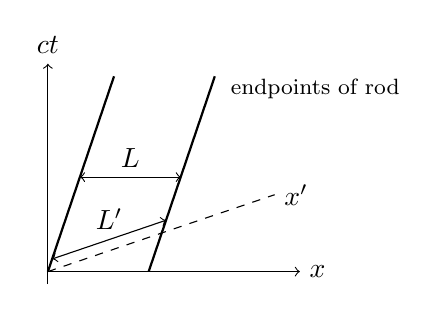
\begin{tikzpicture}[scale=0.8]
	\draw [->] (0, 0) -- (4, 0) node [right] {$x$};
	\draw [->] (0, -0.2) -- (0, 3.3) node [above] {$ct$};
	\draw [thick] (0, 0) -- (1.05, 3.1);
	\draw [thick] (1.6, 0) -- (2.65, 3.1);
	\node at (2.75, 2.9) [right] {\footnotesize endpoints of rod};
	\draw [<->] (0.51, 1.5) -- (2.11, 1.5) node [pos = 0.5, above] {$L$};
	\draw [dashed] (0, 0) -- (3.6, 1.22) node [right] {$x'$};
	\draw [<->] (0.068, 0.2) -- (1.876, 0.815) node [pos = 0.5, above] {$L'$};
\end{tikzpicture}
\end{center}

On the spacetime diagram, $\FF$ measures the rod along a horizontal line of simultaneity, while $\FF'$ measures it along the tilted $x'$ axis -- they are simply measuring \emph{different} pairs of events, which is how both can be right.

\begin{example}[The Train in the Station]
	A train of proper length $2L$ travels at speed $v$, with $\gamma = 2$, through a station whose platform has length $L$. For observers on the platform, the train is contracted to length $2L/\gamma = L$, so for one instant it fits perfectly alongside the platform. But for observers on the train, it is the \emph{platform} that is contracted, to $L/2$, and the train (length $2L$) never comes close to fitting!

	Who is right? Both. `The train fits' means `both ends of the train are alongside the platform \emph{simultaneously}' -- and simultaneity is frame-dependent. The two events `front of train reaches far end of platform' and `back of train passes near end of platform' are simultaneous in the platform frame, but occur in a different order in the train frame. Once stated carefully, there is no contradiction, and the spacetime diagram of the two pairs of world lines shows exactly how the frames disagree.
\end{example}

\subsection{Composition of Velocities}

Suppose a particle moves with constant velocity $u'$ in frame $\FF'$, which moves with velocity $v$ relative to $\FF$. We want to find its velocity $u$ in the frame $\FF$.

In $\FF'$, the world line of the particle is $x' = u't'$. Substituting this into the (inverse) Lorentz transformation laws, we have
$$
u = \frac{x}{t} = \frac{\gamma(x' + vt')}{\gamma(t' + vx'/c^2)} = \frac{u' + v}{1 + u' v/c^2}.
$$
This is the relativistic law for the \vocab{composition of velocities}, replacing the Galilean $u = u' + v$. Some features worth noting:
\begin{enumerate}[label=(\roman*)]
	\item When $u'v \ll c^2$, the denominator is close to $1$ and we recover the Galilean answer -- velocities approximately add at everyday speeds.
	\item If $u' = c$ then $u = (c + v)/(1 + v/c) = c$, for \emph{any} $v$: composing any velocity with the speed of light gives the speed of light, exactly as the second postulate demands.
	\item If $|u'| < c$ and $|v| < c$, then $|u| < c$. Try as we might, we cannot boost a particle past the speed of light by chaining together boosts -- the speed of light is unreachable, not merely unreached.
\end{enumerate}

\begin{example}
	A ship recedes from Earth at $\frac{1}{2}c$ and fires a probe forwards at $\frac{1}{2}c$ relative to itself. Galileo would have the probe moving at $c$; instead,
	$$
	u = \frac{\frac{1}{2}c + \frac{1}{2}c}{1 + \frac{1}{4}} = \frac{4}{5}c.
	$$
	If the probe in turn launches its own sub-probe at $\frac{1}{2}c$, the Earth measures $\frac{(4/5 + 1/2)c}{1 + 2/5} = \frac{13}{14}c$ -- each stage claws closer to $c$, with ever diminishing returns.
\end{example}


\subsection{Geometry of Minkowski Space}

Consider two events $P_1$ and $P_2$ have coordinates $(t_1, x_1)$ and $(t_2, x_2)$ in the frame $\FF$. These events are separated by $\Delta t = t_1 - t_2$ in time and $\Delta x = x_1 - x_2$.

We define the \emph{invariant interval} between $P_1$ and $P_2$ to be
$$
\Delta s^2 = c^2 \Delta t^2 - \Delta x^2.
$$
We say it is invariant because it is the same in all inertial reference frames, that is, it is invariant under Lorentz transformations. This is a direct computation:
\begin{align*}
	c^2 \Delta t'^2 - \Delta x'^2 &= \gamma^2 \left(c\Delta t - \frac{v}{c}\Delta x\right)^2 - \gamma^2 \left(\Delta x - \frac{v}{c}\, c\Delta t\right)^2 \\
	&= \gamma^2 \left(1 - \frac{v^2}{c^2}\right)\left(c^2 \Delta t^2 - \Delta x^2\right) = c^2 \Delta t^2 - \Delta x^2,
\end{align*}
where the cross terms cancel. (In more than one spatial dimension, the interval is $\Delta s^2 = c^2\Delta t^2 - \Delta x^2 - \Delta y^2 - \Delta z^2$, and the transverse coordinates are untouched by the boost.) The invariant interval plays the role in spacetime that squared distance plays in Euclidean geometry: it is the quantity that all observers agree on, even as they disagree about times and lengths separately.

\begin{example}
	In the frame $\FF$, two events are separated by $\Delta x = 3$ light-years and $c\Delta t = 5$ light-years. What does a ship travelling at $v = \frac{3}{5}c$ (so $\gamma = \frac{5}{4}$) between the two events make of them? Applying the Lorentz transformation to the separations,
	$$
	\Delta x' = \gamma\left(\Delta x - \frac{v}{c}\, c\Delta t\right) = \frac{5}{4}(3 - 3) = 0, \quad c\Delta t' = \gamma \left(c \Delta t - \frac{v}{c}\Delta x\right) = \frac{5}{4}\left(5 - \frac{9}{5}\right) = 4.
	$$
	In the ship's frame the two events happen at the \emph{same place} (of course -- the ship is present at both), separated by $4$ years of ship time. And indeed the invariant interval agrees in both frames:
	$$
	\Delta s^2 = 5^2 - 3^2 = 16 = 4^2 - 0^2,
	$$
	with $\Delta s / c = 4$ years being precisely the time experienced aboard -- the \emph{proper time} between the events, computed without ever leaving the frame $\FF$.
\end{example}

It is possible for $\Delta s^2$ to be either positive or negative. If it is positive, we say the events are \emph{timelike} separated, and if it is negative we say they are \emph{spacelike} separated, and if it is zero, we say they are \emph{lightlike} (or \emph{null}) separated. This classification is exactly the light cone structure from before: timelike separated events are in each other's light cones and can influence one another, spacelike separated events cannot, and lightlike separated events can be joined only by a light ray.

Each case has a natural interpretation. For timelike separated events, there is a frame in which the two events happen at the same place, and $\Delta s/c$ is the time between them in that frame -- the \emph{proper time}, of which much more shortly. For spacelike separated events, there is a frame in which they are simultaneous, and $\sqrt{-\Delta s^2}$ is their separation in that frame (the \emph{proper distance}).

There is a nice picture of all this. On a spacetime diagram, the events at fixed invariant interval from the origin form \emph{hyperbolae} $c^2t^2 - x^2 = \text{const}$, with the light cone $x = \pm ct$ as their asymptotes:
\begin{center}
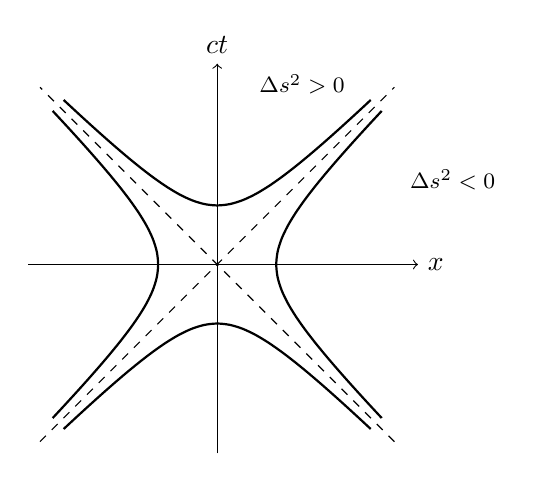
\begin{tikzpicture}[scale=0.75]
	\draw [->] (-3.2, 0) -- (3.4, 0) node [right] {$x$};
	\draw [->] (0, -3.2) -- (0, 3.4) node [above] {$ct$};
	\draw [dashed] (-3, -3) -- (3, 3);
	\draw [dashed] (3, -3) -- (-3, 3);
	\draw [thick, domain=-2.6:2.6, smooth] plot ({\x}, {sqrt(1 + \x*\x)});
	\draw [thick, domain=-2.6:2.6, smooth] plot ({\x}, {-sqrt(1 + \x*\x)});
	\draw [thick, domain=-2.6:2.6, smooth] plot ({sqrt(1 + \x*\x)}, {\x});
	\draw [thick, domain=-2.6:2.6, smooth] plot ({-sqrt(1 + \x*\x)}, {\x});
	\node at (0.55, 3.05) [right] {\footnotesize $\Delta s^2 > 0$};
	\node at (3.1, 1.1) [above right] {\footnotesize $\Delta s^2 < 0$};
\end{tikzpicture}
\end{center}
Lorentz transformations preserve the interval, so they slide events \emph{along} these hyperbolae -- just as rotations of the plane slide points along circles. This is the precise sense in which Lorentz transformations are the `rotations' of spacetime geometry, and we will shortly make the analogy exact using rapidities.

\subsection{4-Vectors}

We can view Minkowski space as a vector space equipped with the \emph{Minkowski inner product}\footnote{This is not an inner product in the normal sense since it's not positive definite}. The coordinates of some event $P$ in the frame $\FF$ can be written as a \emph{4-vector}
$$	
X= \begin{pmatrix}
	ct \\ x \\ y \\ z
\end{pmatrix},
$$
and then the Minkowski inner product is given by
$$
X \cdot Y = X^T \eta Y, \quad \quad \text{where} \quad \eta = \begin{pmatrix}
	1 & 0 & 0 & 0 \\
	0 & -1 & 0 & 0 \\
	0 & 0 & -1 & 0 \\
	0 & 0 & 0 & -1
\end{pmatrix}.
$$
Taking $X \cdot X$ gives the invariant interval between the origin and $P$, and is known as the \emph{Minkowski metric}\footnote{Again, this isn't actually a metric in the normal sense since it's not positive definite}.

More generally, a \vocab{4-vector} is any four-component quantity that transforms under a change of inertial frame in the same way that $X$ does (via the Lorentz transformation matrices of the next subsection). The point of the definition is that the Minkowski inner product of any two 4-vectors is then automatically frame independent -- so building physics out of 4-vectors and their inner products is a machine for generating statements that all inertial observers agree on. We will exploit this repeatedly in the final section.

A quick note on notation, for compatibility with the wider world: the components of a 4-vector are commonly written with a Greek superscript, $X^\mu$ for $\mu = 0, 1, 2, 3$, with $X^0 = ct$ the time component. We will not need the index machinery in this course (it comes into its own in the Part IB `Electromagnetism' and Part II relativity courses), but it is useful to recognise it.

\subsection{The Lorentz Group}

Using $4$-vectors, we can view Lorentz transformations as linear transformations from the coordinates of one inertial frame $\FF$ to another $\FF'$. This would be represented by a $4 \times 4$ matrix $\Lambda$, with
$$
X' = \Lambda X.
$$
Since such transformations must preserve the invariant interval, they must preserve the Minkowski inner product\footnote{These are the analogue of orthogonal matrices for Minkowski space} and hence satisfy
$$
\Lambda^T \eta \Lambda = \eta.
$$
The group of all such matrices is the \emph{Lorentz group}, and is generated by 
$$
\left(\begin{array}{c|ccc}
	1 & 0 & 0 & 0 \\
	\hline 0 & & & \\
	0 & & \mathrm{R} & \\
	0 & & &
	\end{array}\right) 
	\quad \text{and} \quad \left(\begin{array}{cc|cc}
		\gamma & -\gamma v / c & 0 & 0 \\
		-\gamma v / c & \gamma & 0 & 0 \\
		\hline 0 & 0 & 1 & 0 \\
		0 & 0 & 0 & 1
		\end{array}\right),
$$
where the first corresponds to a rotation of space, leaving time intact (so we need $R$ to be orthogonal), and the second corresponds to a Lorentz boost along the $x$ direction.

\begin{remark}
	Taking determinants of $\Lambda^T \eta \Lambda = \eta$ gives $(\det \Lambda)^2 = 1$, so $\det \Lambda = \pm 1$, and one can also show $|\Lambda^0_{\;0}| \geq 1$. The physically relevant transformations -- those continuously connected to the identity -- have $\det \Lambda = +1$ and $\Lambda^0_{\;0} \geq 1$: they preserve both spatial orientation and the direction of time. The remaining components of the group involve spatial reflections or time reversal.
\end{remark}

\subsection{Rapidities}

Consider a $2 \times 2$ matrix corresponding to a Lorentz boost by $v$ in the $x$ direction. Then if $\beta = v/c$, we have
$$
\Lambda[\beta] = \begin{pmatrix}
	\gamma & -\gamma \beta \\
	-\gamma \beta & \gamma
\end{pmatrix}
$$
and the composition law $\Lambda[\beta_1] \Lambda[\beta_2] = \Lambda\left[\frac{\beta_1 + \beta_2}{1 + \beta_1 \beta_2}\right]$,
which is exactly our composition law from before.

A slightly nicer way to deal with this is with \emph{rapidities}.
We define the \emph{rapidity} of a Lorentz boost $\phi$ such that
$$
\beta = \tanh \phi, \quad \gamma = \cosh \phi,\quad \gamma \beta = \sinh \phi.
$$
Then
$$
\Lambda[\beta] = \begin{pmatrix}
	\cosh \phi & - \sinh \phi \\
	-\sinh \phi & \cosh \phi 
\end{pmatrix} = \Lambda(\phi),
$$
and also
$$
\Lambda(\phi_1) \Lambda(\phi_2) = \Lambda(\phi_1 + \phi_2),
$$
which is much nicer. This also shows that Lorentz boosts correspond to hyperbolic rotations in spacetime, just as the rotation matrices (with $\cos$ and $\sin$) represent ordinary rotations of space. The trigonometry of Minkowski space is hyperbolic trigonometry.

Rapidities also give the slickest possible derivation of the composition of velocities: composing boosts of rapidities $\phi_1$ and $\phi_2$ gives a boost of rapidity $\phi_1 + \phi_2$, whose velocity is
$$
\frac{u}{c} = \tanh(\phi_1 + \phi_2) = \frac{\tanh \phi_1 + \tanh\phi_2}{1 + \tanh\phi_1 \tanh\phi_2} = \frac{v_1/c + v_2/c}{1 + v_1v_2/c^2},
$$
by the addition formula for $\tanh$ -- our composition law falls straight out. And since $\tanh$ maps $\R$ to $(-1, 1)$, no amount of adding rapidities ever reaches the speed of light: on the rapidity scale, velocities add plainly, and $c$ sits at infinity.


\section{Relativistic Physics}

Having rebuilt the geometry of space and time, we now rebuild \emph{dynamics}: velocity, momentum, energy and force, all in a form that respects Lorentz transformations. The guiding principle is to phrase everything in terms of 4-vectors and Lorentz invariants, so that the physics manifestly takes the same form in every inertial frame. The payoff comes at the end of the section, where conservation of 4-momentum will let us analyse particle collisions, decays and creation processes with remarkable ease.

\subsection{Proper Time}

To do kinematics, it helps to have a notion of time that all observers can agree on. We do this by defining \vocab{proper time} $\tau$, which is the time experienced by a particle in its own reference frame. It is given by
$$
\Delta \tau = \frac{\Delta s}{c}
$$
along the particle's world line, in all reference frames -- this is well defined precisely because $\Delta s$ is Lorentz invariant. (For a massive particle, successive events on the world line are timelike separated, so $\Delta s^2 > 0$ and the proper time is real.)

We can relate proper time to the time measured in any particular frame by considering small changes. If $\vv u$ is the velocity of the particle in the frame $\FF$, we get
$$
\dd \tau = \frac{1}{c} \dd s = \frac{1}{c} \sqrt{c^2 \dd t^2 - |\dd\vv x|^2} = \sqrt{1 - u^2/c^2}\dd t,
$$
so
$$
\frac{\dd t}{\dd \tau} = \gamma_u, \quad \text{where } \gamma_u = \frac{1}{\sqrt{1 - u^2/c^2}}.
$$
Note that $\gamma_u$ here is built from the \emph{particle's} speed in $\FF$, which need not be constant. We can then get the total time experienced by a particle along a segment of its world line as
$$
T = \int \dd \tau = \int \frac{1}{\gamma_u} \dd t \leq \int \dd t.
$$
So of all observers passing through the same two events, the one who experiences the most time is the one moving inertially -- a restatement of the twin paradox.

\begin{example}
	An astronaut spends six months on the International Space Station, orbiting at about $\SI{7.7}{\kilo\meter\per\second}$. Over the mission, the proper time deficit relative to mission control is
	$$
	\Delta t - \Delta \tau = \left(1 - \frac{1}{\gamma}\right)\Delta t \approx \frac{v^2}{2c^2}\, \Delta t \approx \frac{(7.7 \times 10^3)^2}{2(3\times 10^8)^2} \times \SI{1.6e7}{\second} \approx \SI{5}{\milli\second}.
	$$
	The astronaut returns five milliseconds younger than if they had stayed home -- a small effect, but one routinely confirmed by flying atomic clocks around the world.
\end{example}

\subsection{4-Velocity}

Using proper time, we can parametrise the trajectory of a particle using a $4$-vector
$$
X(\tau) = \begin{pmatrix}
	ct(\tau) \\
	\vv x(\tau)
\end{pmatrix},
$$
the \emph{4-position}, and then define the \vocab{$4$-velocity} as its derivative with respect to proper time:
$$
U = \frac{\dd X}{\dd \tau} = \begin{pmatrix}
	c \dd t/\dd\tau \\
	\dd \vv x / \dd \tau
\end{pmatrix}
= \frac{\dd t}{\dd\tau} \begin{pmatrix}
	c \\ \vv u
\end{pmatrix} = \gamma_u \begin{pmatrix}
	c \\ \vv u
\end{pmatrix},
$$
where $\vv u = \dd \vv x/ \dd t$ is the ordinary velocity in the frame. The reason to differentiate with respect to $\tau$ rather than $t$ is that $\tau$ is an invariant: since $X' = \Lambda X$ and $\tau$ is frame independent, the 4-velocity genuinely transforms as a 4-vector, $U' = \Lambda U$. (The naive candidate $\dd X/\dd t$ transforms in no nice way at all.)

Like any 4-vector, $U$ has an invariant inner product with itself. Easiest computed in the particle's rest frame, where $U = (c, \vv 0)$:
$$
U \cdot U = c^2,
$$
and indeed in a general frame $U \cdot U = \gamma_u^2 (c^2 - |\vv u|^2) = c^2$. Every particle traverses spacetime with `4-speed' $c$.

\subsection{Transforming Velocities \& Aberration}

Since $U' = \Lambda U$, transforming velocities between frames is now just linear algebra -- which lets us generalise our composition law to velocities in arbitrary directions. Suppose in frame $\FF$ a particle moves with speed $u$ at angle $\theta$ to the $x$-axis, in the $(x,y)$ plane, and let $\FF'$ move at speed $v$ in the $x$ direction as usual. Applying the boost matrix to $U = \gamma_u(c, u\cos\theta, u \sin\theta, 0)^T$:
$$
\begin{pmatrix}
	\gamma_{u'} c \\ \gamma_{u'} u' \cos\theta' \\ \gamma_{u'} u' \sin \theta' \\ 0
\end{pmatrix} = \begin{pmatrix}
	\gamma_v & -\gamma_v v/c & 0 & 0 \\
	-\gamma_v v/c & \gamma_v & 0 & 0 \\
	0 & 0 & 1 & 0 \\
	0 & 0 & 0 & 1
\end{pmatrix}\begin{pmatrix}
	\gamma_u c \\ \gamma_u u \cos\theta \\ \gamma_u u \sin\theta \\ 0
\end{pmatrix}.
$$
Dividing the second row by the first eliminates the $\gamma$ factors and gives
$$
u' \cos \theta' = \frac{u \cos\theta - v}{1 - \frac{uv}{c^2}\cos\theta},
$$
the familiar composition law applied to the parallel component. Dividing the third row by the second gives
$$
\tan \theta' = \frac{u \sin \theta}{\gamma_v (u \cos\theta - v)},
$$
which describes \vocab{aberration}: the direction of motion of a particle depends on the motion of the observer. There is a Newtonian part to this effect -- walk through vertical rain and it appears to slant towards you -- but the $\gamma_v$ factor is genuinely relativistic. For light ($u = c$), aberration causes the apparent positions of stars to shift annually as the Earth swings around its orbit, an effect measured long before relativity explained it correctly.

\subsection{4-Momentum \& Relativistic Energy}

With the 4-velocity in hand, we can define the relativistic analogue of momentum.

\begin{definition}[4-Momentum]
	For a particle of mass $m$, the \vocab{$4$-momentum} is
	$$
	P = mU = \begin{pmatrix}
		mc \gamma_u \\
		m \gamma_u \vv u
	\end{pmatrix}.
	$$
\end{definition}

The spatial components of $P$ give us the \emph{relativistic $3$-momentum}, $\vv p = m \gamma_u \vv u$, which is the Newtonian momentum corrected by a factor of $\gamma_u$ -- note that $|\vv p| \to \infty$ as $|\vv u| \to c$. The fundamental law of relativistic dynamics is that \emph{$4$-momentum is conserved}: for a system of particles the total $4$-momentum (the sum of the individual $4$-momenta) is unchanged by collisions and interactions, in the absence of external forces. This single conservation law packages together the conservation of momentum \emph{and} of energy, as we now see by interpreting the time component.

Expanding $P^0$ for speeds small compared to $c$,
$$
P^0 = m\gamma_u c = \frac{1}{c}\left(mc^2 + \frac{1}{2}m|\vv u|^2 + \cdots\right).
$$
The second term is the Newtonian kinetic energy, so we recognise $P^0 c$ as an energy.

\begin{definition}[Relativistic Energy]
	The \vocab{relativistic energy} of a particle is $E = P^0 c = m\gamma_u c^2$, so that
	$$
	P = \begin{pmatrix}
		E/c \\ \vv p
	\end{pmatrix}, \quad \text{and} \quad E = mc^2 + \underbrace{(\gamma_u - 1)mc^2}_{\text{kinetic energy}}.
	$$
\end{definition}

For a stationary particle we have the most famous equation in physics:
$$
E = mc^2.
$$
Mass is a form of energy -- and an enormously concentrated one, with $c^2 \approx \SI{9e16}{\joule\per\kilogram}$ as the exchange rate. In relativity, mass is \emph{not} separately conserved: it can be converted to kinetic energy and back, as happens in nuclear reactions and particle colliders, and only the total energy (including mass energy) is conserved.

Since we can calculate the Lorentz invariant quantity $P \cdot P$ in the particle's rest frame, we have
$$
P \cdot P = \frac{E^2}{c^2} - |\vv p|^2 = m^2 c^2,
$$
so generally we have the \vocab{energy-momentum relation}
$$
E^2 = |\vv p|^2 c^2 + m^2 c^4.
$$
This invariant is the workhorse of collision problems: given any 4-momentum (perhaps a sum over several particles), dotting it with itself produces frame-independent information.

\emph{Massless particles.} For particles that have zero mass (like photons), we cannot define proper time or 4-velocity -- but we can still perfectly well assign them a 4-momentum, with $P \cdot P = 0$. Such particles travel at the speed of light, along lightlike trajectories, and can still carry momentum and energy, related by $E = |\vv p| c$. Thus
$$
P = \frac{E}{c} \begin{pmatrix}
	1 \\ \vv n
\end{pmatrix},
$$
where $\vv n$ is a unit vector in the direction of propagation. Quantum mechanics supplies the energy in terms of the light's frequency $f$ (or wavelength $\lambda = c/f$) via the \emph{Planck relation} $E = hf = hc/\lambda$, where $h$ is Planck's constant.

\subsection{The Relativistic Doppler Effect}

Suppose a source of light recedes from an observer at speed $v$, emitting light of frequency $f'$ (as measured in the source's own rest frame). What frequency does the observer measure? Two effects stack: successive wave crests are emitted at intervals lengthened by time dilation, \emph{and} each crest is emitted from further away than the last, adding travel time.

Quantitatively: in the observer's frame, the source's clock ticks slowly, so crests are emitted at intervals $\gamma T'$, where $T' = 1/f'$. Between successive emissions the source recedes a further distance $v \gamma T'$, delaying the later crest's arrival by $v\gamma T'/c$. So crests arrive separated by
$$
T = \gamma T' + \frac{v \gamma T'}{c} = T' \gamma\left(1 + \frac{v}{c}\right) = T'\sqrt{\frac{1 + v/c}{1 - v/c}},
$$
and hence the observed frequency is
$$
f = f' \sqrt{\frac{1 - v/c}{1 + v/c}}.
$$
For a receding source, $f < f'$: the light is shifted towards the red end of the spectrum (\emph{redshift}). For an approaching source, replace $v$ with $-v$ to get a \emph{blueshift}. An elegant alternative derivation: apply a Lorentz boost to the photon's 4-momentum, $E = \gamma(E' - vE'/c \cdot 1)$ for a photon emitted backwards, and use $E = hf$ -- the same factor drops out.

Note that even the \emph{transverse} Doppler effect (source moving perpendicular to the line of sight) is nontrivial in relativity, giving $f = f'/\gamma$ purely from time dilation, with no Newtonian counterpart.

The Doppler effect is a workhorse of astronomy: the redshifts of spectral lines tell us how fast stars and galaxies move along our line of sight, and the systematic redshift of distant galaxies -- Hubble's observation that essentially everything is receding from us -- is the observational cornerstone of the expanding universe.

It also gives a satisfying second look at the twin paradox. Suppose the travelling twin Alice sends Bob a light pulse every year of \emph{her} time. On the outward leg, Bob receives the pulses at the slowed rate $\sqrt{(1-\beta)/(1+\beta)}$ per year; after her turnaround, at the sped-up rate $\sqrt{(1+\beta)/(1-\beta)}$. But here is the asymmetry: Alice's turnaround changes what she \emph{sends} at her half-way point, while Bob only starts \emph{receiving} the sped-up pulses late in the trip, when the last outbound pulse finally crawls to him. Counting the pulses each twin receives over the whole journey (a pleasant exercise) reproduces exactly the asymmetric ageing -- no frames or lines of simultaneity required, just counting flashes of light.

\subsection{4-Force}

We can now write down the relativistic version of Newton's second law. The natural formulation uses proper time and 4-vectors throughout.

\begin{definition}[4-Force]
	The \vocab{4-force} on a particle with 4-momentum $P$ is
	$$
	F = \frac{\dd P}{\dd\tau}.
	$$
\end{definition}

Since $P$ is a 4-vector and $\tau$ is invariant, $F$ is a genuine 4-vector, transforming as $F' = \Lambda F$ -- so if this law holds in one inertial frame, it holds in all of them, exactly as the principle of relativity requires. Writing out the components in a frame where the particle has velocity $\vv u$, and comparing with $P = (E/c, \vv p)$, we can express the 4-force in terms of the ordinary 3-force $\vv F = \dd\vv p/\dd t$:
$$
F = \gamma_u \begin{pmatrix}
	\vv F \cdot \vv u / c \\
	\vv F
\end{pmatrix},
$$
where the factors of $\gamma_u$ come from $\dd t/\dd\tau = \gamma_u$. The two components carry familiar content:
$$
\frac{\dd E}{\dd t} = \vv F \cdot \vv u, \quad \frac{\dd \vv p}{\dd t} = \vv F,
$$
that is, the rate of working of the force equals the rate of change of (relativistic) energy, and force is the rate of change of (relativistic) momentum -- Newtonian mechanics upgraded, with $\gamma$ factors hiding inside $E$ and $\vv p$.

For a particle of constant mass we can also write $F = mA$, where
$$
A = \frac{\dd U}{\dd\tau}
$$
is the \emph{4-acceleration}. Differentiating the identity $U \cdot U = c^2$ with respect to $\tau$ gives
$$
U \cdot A = 0,
$$
so the 4-acceleration is always Minkowski-orthogonal to the 4-velocity. In the instantaneous rest frame, $U = (c, \vv 0)$ and $A = (0, \vv a)$, making the orthogonality manifest.

\begin{example}[Motion Under a Constant Force]
	Push a particle of mass $m$ with a constant 3-force $F$ (in one dimension) forever. Newtonian mechanics says $v = Ft/m$ grows without bound; what does relativity say? We have $\dd p/\dd t = F$, so starting from rest,
	$$
	p = m \gamma_u u = Ft \implies u = \frac{Ft/m}{\sqrt{1 + (Ft/mc)^2}},
	$$
	solving for $u$. At early times ($Ft \ll mc$) this is the Newtonian $u \approx Ft/m$; at late times $u \to c$ but never reaches it -- the momentum grows linearly forever, but ever more of the `push' goes into the $\gamma$ factor rather than into speed. Constant proper acceleration traces out a \emph{hyperbola} on the spacetime diagram, asymptotic to a light ray: one more instance of hyperbolae being relativity's circles.
\end{example}

\subsection{Particle Collisions \& Decays}

We finish the course with relativistic particle physics -- the study of collisions, decays and creation of particles, where conservation of total 4-momentum
$$
P = \begin{pmatrix} E/c \\ \vv p\end{pmatrix}
$$
does essentially all of the work. A frame that makes calculations dramatically easier:

\begin{definition}[Centre of Momentum Frame]
	The \vocab{centre of momentum frame} of a system of particles is an inertial frame in which the total 3-momentum vanishes, $\sum_i \vv p_i = \vv 0$.
\end{definition}

Such a frame exists for any system except one consisting entirely of massless particles moving in a single direction. It is the relativistic analogue of the centre of mass frame from Newtonian collisions.

\begin{remark}
	A closely related tool: for any system with total 4-momentum $P_{\text{tot}}$, the quantity
	$$
	M_{\text{inv}}^2 c^2 = P_{\text{tot}} \cdot P_{\text{tot}}
	$$
	defines the \emph{invariant mass} of the system -- it is frame independent, equal to the total energy in the centre of momentum frame divided by $c^2$, and (because 4-momentum is conserved) unchanged by any decay or collision the system undergoes. Note that the invariant mass of a system is generally \emph{greater} than the sum of the rest masses of its constituents, the excess being internal kinetic energy. Reconstructing invariant masses from measured decay products is how new particles are actually discovered.
\end{remark}

\subsubsection{Particle Decay}

Suppose a particle of mass $m_1$ decays into two particles of masses $m_2$ and $m_3$. Conservation of 4-momentum reads
$$
P_1 = P_2 + P_3,
$$
which contains both $E_1 = E_2 + E_3$ and $\vv p_1 = \vv p_2 + \vv p_3$. Work in the rest frame of the decaying particle (its own centre of momentum frame). There, $E_1 = m_1 c^2$, and using the energy-momentum relation for the products,
$$
m_1 c^2 = \sqrt{|\vv p_2|^2 c^2 + m_2^2 c^4} + \sqrt{|\vv p_3|^2 c^2 + m_3^2 c^4} \geq m_2 c^2 + m_3 c^2.
$$
So decay is possible only if
$$
m_1 \geq m_2 + m_3
$$
-- a particle can only decay into products whose total mass does not exceed its own, with the excess mass converted into the kinetic energy of the products. (Mass is not conserved!)

\begin{example}[Higgs Decay to Photons]
	One of the decay channels in which the Higgs boson was discovered at the LHC is a decay into two photons, $h \to \gamma\gamma$ (allowed, since $m_\gamma = 0$). In the Higgs rest frame,
	$$
	P_h = \begin{pmatrix} m_h c \\ \vv 0 \end{pmatrix} = P_{\gamma_1} + P_{\gamma_2}.
	$$
	The spatial components force $\vv p_{\gamma_1} = -\vv p_{\gamma_2}$: the photons fly off back-to-back. Since $E_\gamma = |\vv p_\gamma| c$ for each photon, the two photons have equal energies, and the time component then gives
	$$
	E_{\gamma_1} = E_{\gamma_2} = \frac{1}{2}m_h c^2.
	$$
	All of the Higgs mass is converted into electromagnetic energy. Experimentally one runs this backwards: measuring the photon pair and reconstructing the invariant $(P_{\gamma_1} + P_{\gamma_2})\cdot(P_{\gamma_1} + P_{\gamma_2}) = m_h^2c^2$ reveals the mass of the particle that decayed.
\end{example}

\begin{example}[Photon Emission \& Recoil]
	An atom of mass $m$, at rest, drops to a lower energy state of mass $m' < m$ (the internal energy released being $\Delta E = (m - m')c^2$), emitting a single photon. Naively the photon should carry energy $\Delta E$ -- but the atom must recoil to conserve momentum, and the recoil steals some energy. Conservation of 4-momentum gives $P_{\text{atom}} = P_\gamma + P'_{\text{atom}}$, so isolating and squaring the final atom's 4-momentum,
	$$
	m'^2 c^2 = (P_{\text{atom}} - P_\gamma)\cdot(P_{\text{atom}} - P_\gamma) = m^2c^2 - 2 P_{\text{atom}} \cdot P_\gamma = m^2 c^2 - 2m E_\gamma,
	$$
	using $P_\gamma \cdot P_\gamma = 0$ and evaluating $P_{\text{atom}}\cdot P_\gamma = mE_\gamma$ in the rest frame. Hence
	$$
	E_\gamma = \frac{(m^2 - m'^2)c^2}{2m} = \Delta E \left(1 - \frac{\Delta E}{2mc^2}\right).
	$$
	The photon carries slightly \emph{less} than the transition energy, the deficit being carried off as the atom's recoil kinetic energy. For optical transitions the correction is minuscule ($\Delta E/mc^2 \sim 10^{-10}$), but for gamma-ray emission from nuclei it matters enormously -- and clever ways around the recoil (the M\"ossbauer effect) enabled some of the most precise tests of relativity ever performed.
\end{example}

\subsubsection{Particle Scattering}

Next, consider an \emph{elastic} collision: two identical particles of mass $m$ collide and retain their identities, so
$$
P_1 + P_2 = P_3 + P_4.
$$
Set up the standard experiment in the lab frame $\FF$: particle 1 moves with speed $u$ along the $x$-axis and strikes particle 2 at rest, after which the particles move off at angles $\theta$ and $\phi$ to the axis.

The trick is to analyse the collision in the centre of momentum frame $\FF'$, which moves at some speed $v$ along the $x$-axis relative to the lab. In $\FF'$, the two particles approach head-on with equal and opposite momenta, and (comparing the time components of 4-momentum before and after) they must also \emph{recede} with equal and opposite momenta of the same magnitude, each with the same speed $v$ as before. The only freedom is the scattering angle $\theta'$:
$$
P_3' = \begin{pmatrix} m\gamma_v c \\ m \gamma_v v \cos\theta' \\ m \gamma_v v \sin \theta' \\ 0\end{pmatrix}, \quad P_4' = \begin{pmatrix} m\gamma_v c \\ -m \gamma_v v \cos\theta' \\ -m \gamma_v v \sin \theta' \\ 0\end{pmatrix}.
$$
Now boost back to the lab frame with the inverse Lorentz transformation. The incoming particle's speed matches the collision setup provided
$$
u = \frac{2v}{1 + v^2/c^2}
$$
(the composition of $v$ with $v$, naturally, since the target is at rest in the lab and moves at $v$ in $\FF'$). Transforming $P_3'$ and $P_4'$ and taking ratios of components to extract the angles, the half-angle formulae give
$$
\tan \theta = \frac{\sin\theta'}{\gamma_v (1 + \cos\theta')} = \frac{1}{\gamma_v} \tan \frac{\theta'}{2}, \quad
\tan \phi = \frac{\sin\theta'}{\gamma_v (1 - \cos\theta')} = \frac{1}{\gamma_v} \cot \frac{\theta'}{2}.
$$
The individual angles depend on $\theta'$, which is not determined by conservation laws alone -- but their product is universal:
$$
\tan\theta \tan\phi = \frac{1}{\gamma_v^2}.
$$
In the Newtonian limit $\gamma_v \to 1$ we recover $\tan\theta\tan\phi = 1$, i.e.\ $\theta + \phi = \pi/2$: the equal-mass particles separate at right angles, exactly as we found in Section~\ref{sec:systems}. Relativistically, $\tan\theta\tan\phi < 1$, so the opening angle between the outgoing particles is \emph{less} than a right angle -- fast collisions throw both products forward, and measuring this closing-up of the angle is a direct test of special relativity.

\begin{example}[Compton Scattering]
	A lovely application of 4-momentum bookkeeping: scatter a photon off an electron (mass $m$) at rest, and ask how the photon's wavelength changes. Let the incoming photon have energy $E$, the outgoing photon energy $E'$ at angle $\theta$ to the incident direction, and let the electron recoil with 4-momentum $P_e'$. Conservation says
	$$
	P_\gamma + P_e = P_\gamma' + P_e'.
	$$
	We don't care about the electron's recoil, so isolate it and take the invariant square:
	$$
	P_e' \cdot P_e' = (P_\gamma + P_e - P_\gamma') \cdot (P_\gamma + P_e - P_\gamma') .
	$$
	The left side is $m^2c^2$. Expanding the right side using $P_\gamma \cdot P_\gamma = P_\gamma' \cdot P_\gamma' = 0$ and $P_e \cdot P_e = m^2c^2$,
	$$
	m^2 c^2 = m^2c^2 + 2 P_\gamma \cdot P_e - 2 P_\gamma' \cdot P_e - 2 P_\gamma \cdot P_\gamma',
	$$
	and computing each inner product in the lab frame (where $P_e = (mc, \vv 0)$):
	$$
	P_\gamma \cdot P_e = mE, \quad P_\gamma' \cdot P_e = mE', \quad P_\gamma \cdot P_\gamma' = \frac{EE'}{c^2}(1 - \cos\theta).
	$$
	Substituting and tidying up,
	$$
	\frac{1}{E'} - \frac{1}{E} = \frac{1 - \cos\theta}{mc^2},
	$$
	or, in terms of wavelengths via the Planck relation $E = hc/\lambda$,
	$$
	\lambda' - \lambda = \frac{h}{mc}(1 - \cos \theta).
	$$
	The scattered light is shifted to longer wavelengths, by an amount depending only on the scattering angle and the universal length $h/mc$ (the \emph{Compton wavelength} of the electron). Compton's measurement of exactly this shift in 1923 was decisive evidence that light really does carry momentum in particle-like quanta.
\end{example}

\subsubsection{Particle Creation \& Threshold Energies}

Finally, creation of new particles: collide two particles of mass $m$ fast enough, and the excess kinetic energy can be converted into the mass of a new particle:
$$
P_1 + P_2 = P_3 + P_4 + P_5,
$$
where particles 3 and 4 have mass $m$ and the newly created particle 5 has mass $M$.

Work in the centre of momentum frame, where the two initial particles approach with equal speeds $v$. The total 4-momentum is
$$
P_1 + P_2 = \begin{pmatrix} 2m \gamma_v c \\ \vv 0\end{pmatrix},
$$
and after the collision, the total energy is $E_3 + E_4 + E_5 \geq (2m + M)c^2$, with equality when all three products are at rest. So creation is possible only if
$$
2m\gamma_v c^2 \geq (2m + M)c^2, \quad \text{i.e.} \quad \gamma_v \geq 1 + \frac{M}{2m},
$$
or in terms of kinetic energy: the initial kinetic energy in the centre of momentum frame must be at least $Mc^2$. This is the \vocab{threshold energy} for the process -- entirely reasonable: every joule of kinetic energy in this frame is available for making mass.

The situation is dramatically different in a \emph{fixed-target} experiment, where one initial particle is at rest in the lab. The lab frame moves at speed $v$ relative to the centre of momentum frame, so the moving particle has speed $u = 2v/(1 + v^2/c^2)$, for which one can check the useful identity
$$
\gamma_u = 2\gamma_v^2 - 1.
$$
At threshold, $\gamma_v = 1 + M/2m$, so we require
$$
\gamma_u \geq 2\left(1 + \frac{M}{2m}\right)^2 - 1 = 1 + \frac{2M}{m} + \frac{M^2}{2m^2},
$$
that is, an initial kinetic energy of
$$
m(\gamma_u - 1)c^2 \geq \left(2 + \frac{M}{2m}\right)Mc^2.
$$
This is far more than $Mc^2$ when $M \gg m$: most of the beam's energy is wasted on the kinetic energy that the products are forced to carry (the total momentum is nonzero and must be conserved). This is precisely why modern particle physics is done with \emph{colliders}, smashing two beams together head-on -- the lab \emph{is} the centre of momentum frame, and every unit of beam energy is available for creating new particles. To create a Higgs boson ($M \approx 130$ proton masses) with a fixed-target proton experiment would require a beam energy hundreds of times larger than the LHC's colliding beams need.

And that -- from Newton's laws to the design principles of the Large Hadron Collider -- is where we end the course.

\end{document}